\chapter{Rocketry}


Rockets propel hot gases, which recreates an equal an opposite reaction which pushes it forwards, even in a vacuum. 

Even without anything to push against, the rocket can still move forward thanks to Newton's Third Law. 

Imagine a spacecraft with a bowling ball attached to the back. If that spacecraft exerts a force to throw the bowling ball backwards, the ball will exert a force on the ship, moving it forwards. 


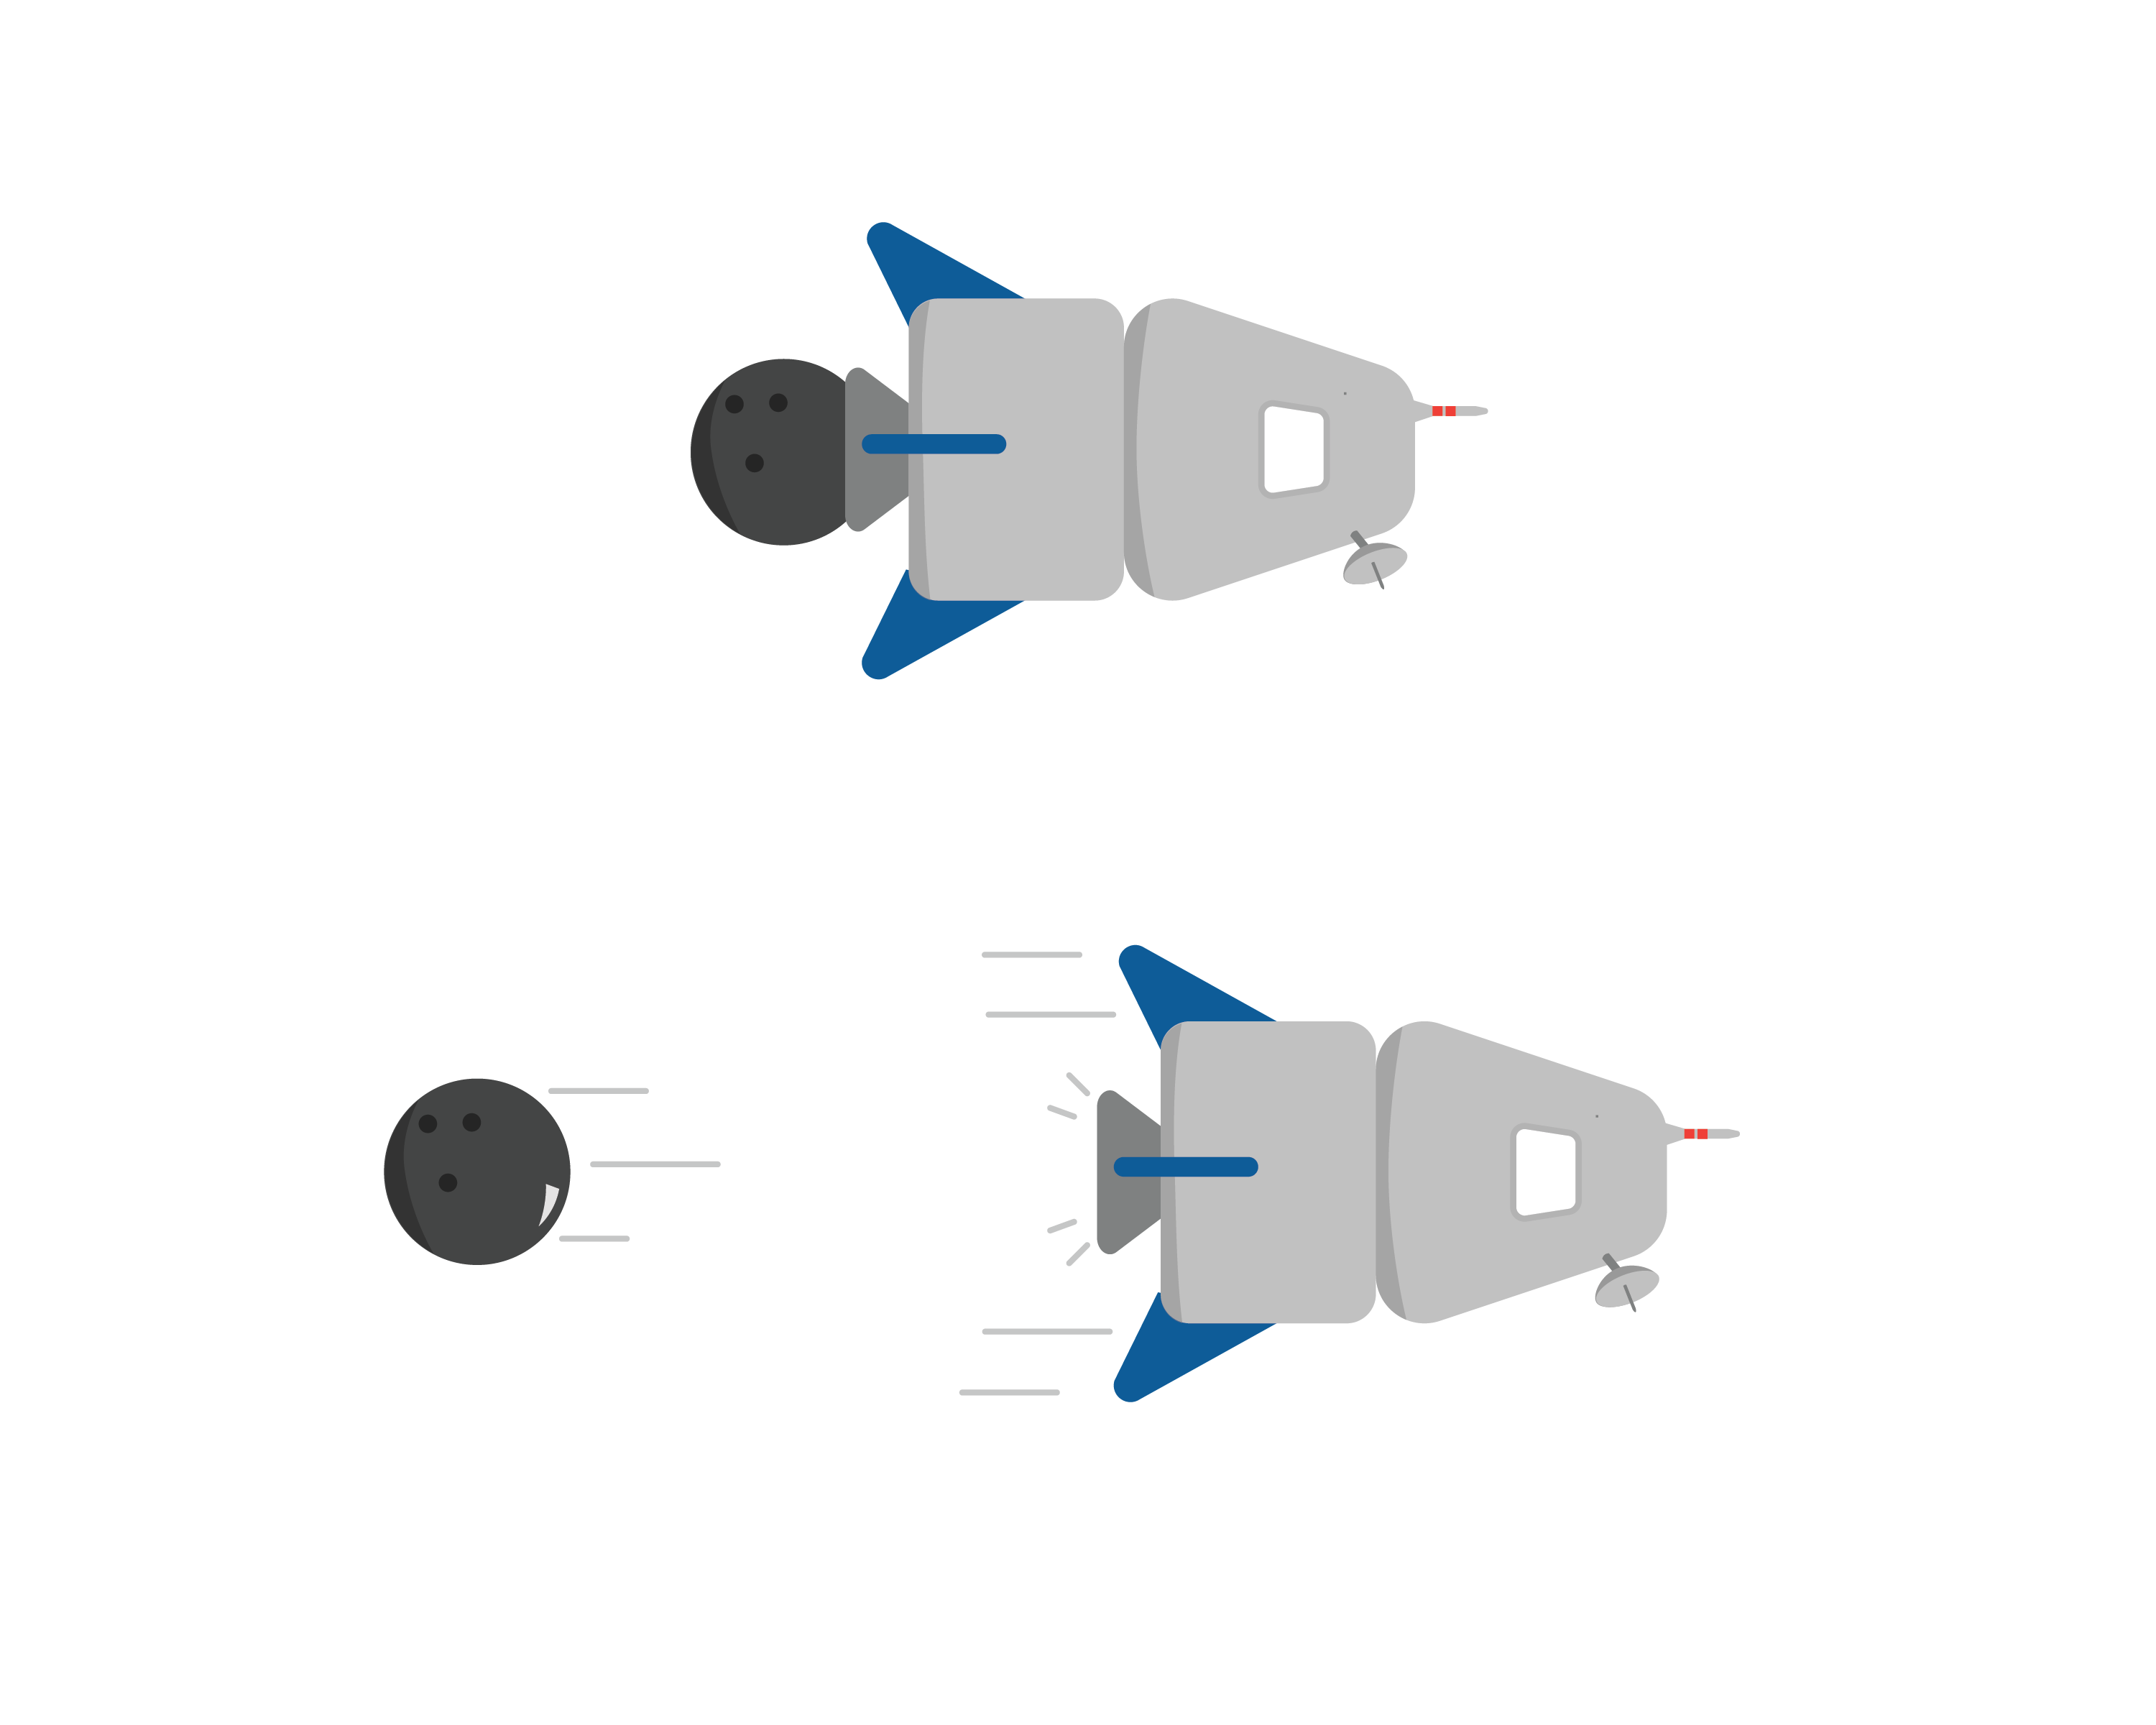
\includegraphics[width=0.75\textwidth]{thirdLaw.png}

Instead of a bowling ball, real-life rockets usually "throw" particles of hot gas at very high speeds. Rockets carry their own oxidizer to provide oxygen to allow fuel to burn. 

\section{Types of rocket motors}

There are two main types of chemical rockets. 

One type is a \newterm{Solid Fuel Rocket}, which ignites a solid fuel-oxidizer mix. Once the solid fuel is ignited it can't be stopped until all of the fuel is exhausted.


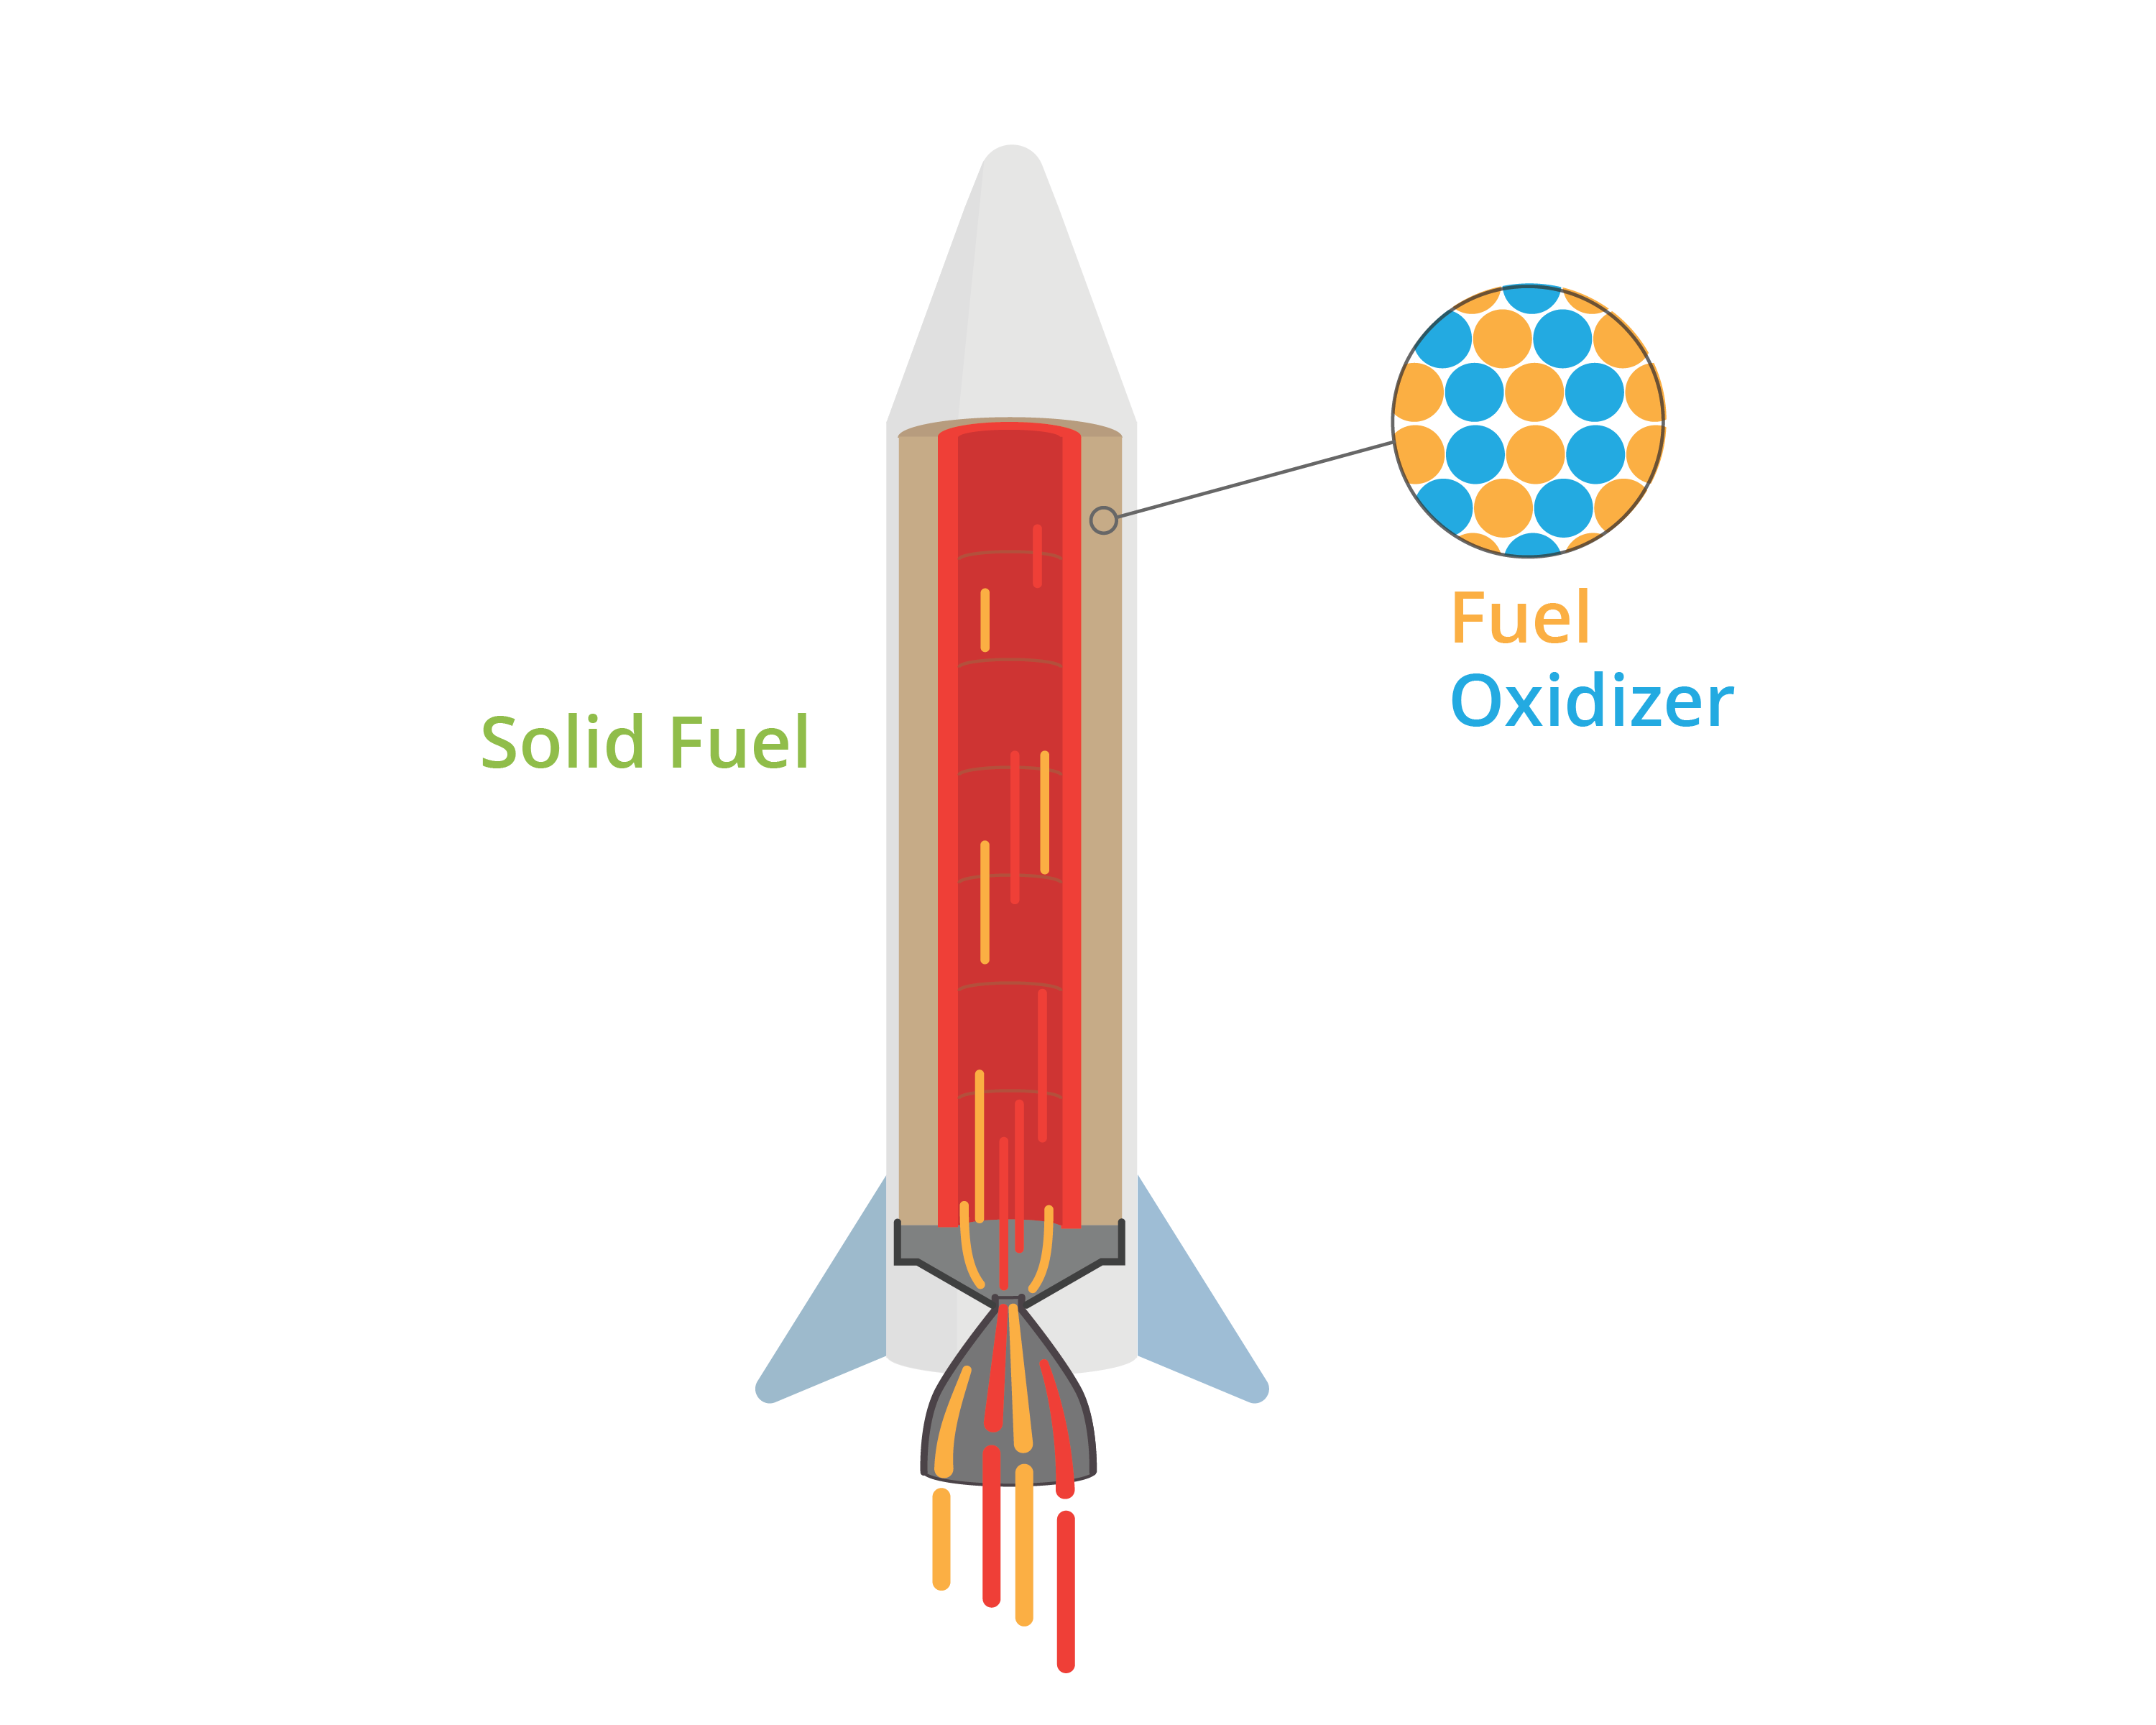
\includegraphics[width=0.75\textwidth]{solid.png}

The other main type of chemical rocket is called a \newterm{Liquid Fuel Rocket}

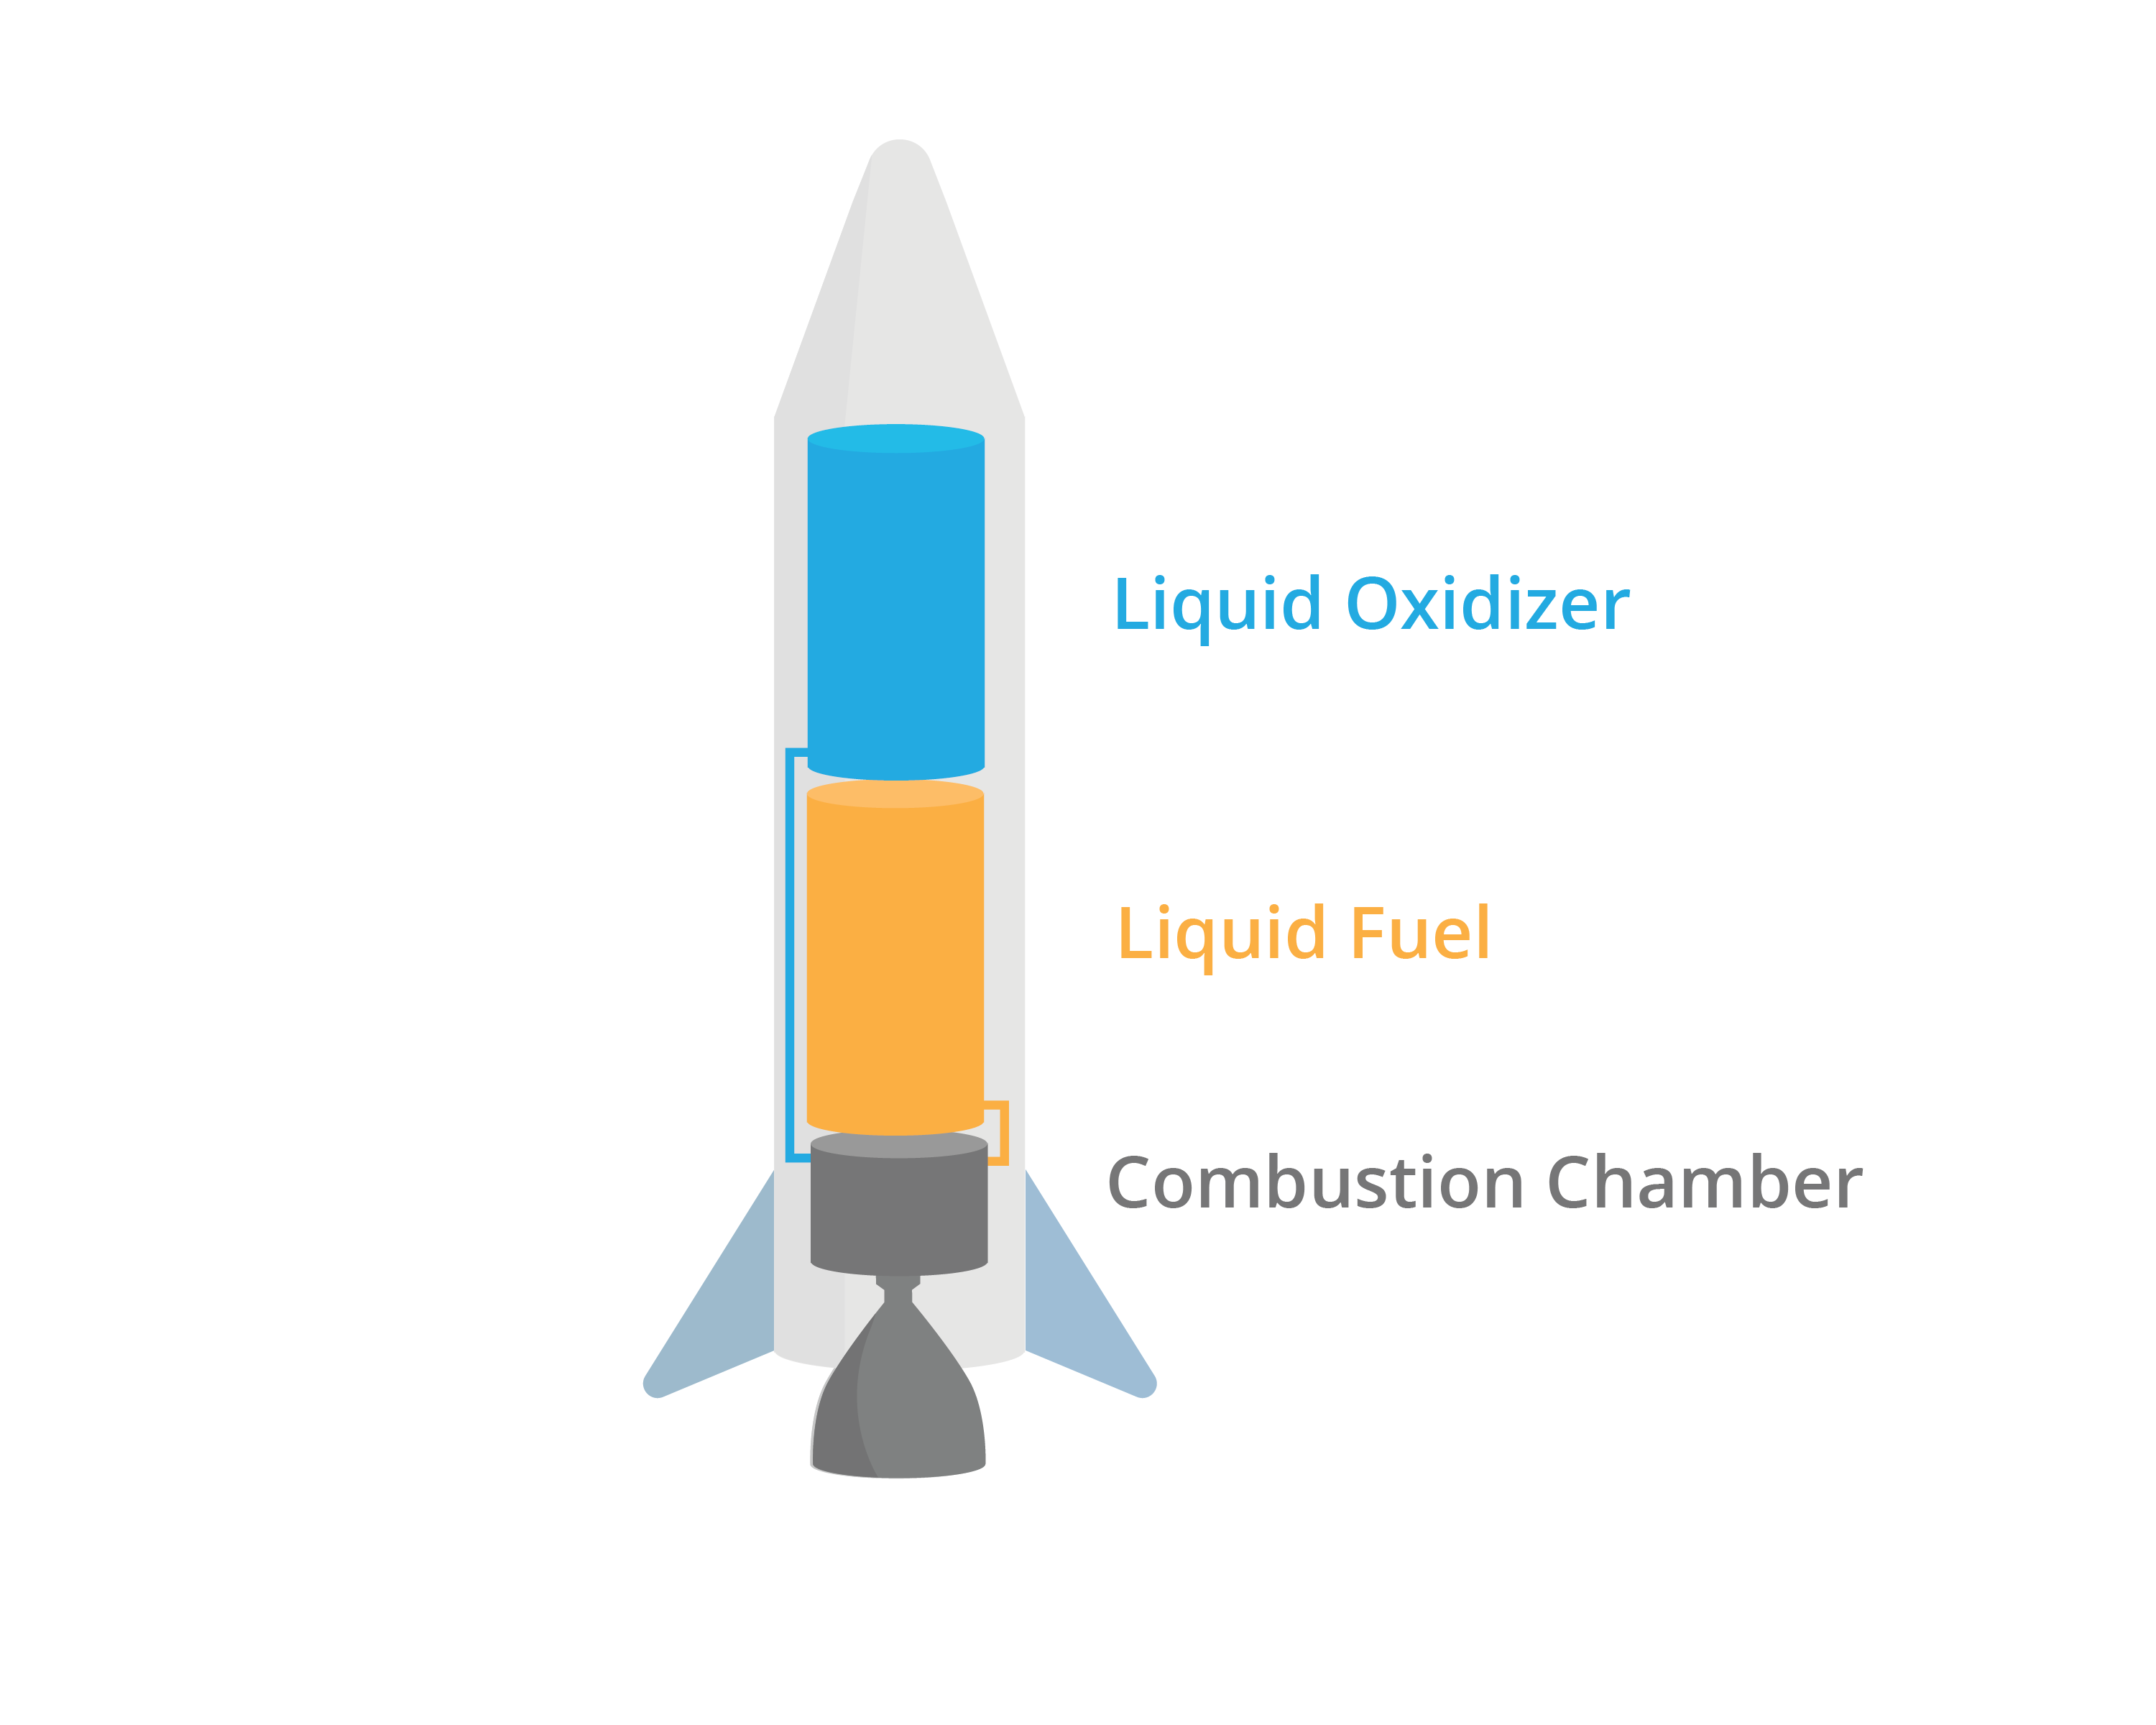
\includegraphics[width=0.75\textwidth]{liquid.png}

Liquid fuel rockets contain separate tanks for liquid fuel and liquid oxygen. Fuel pumps bring them both to a combustion chamber where they ignite and exit the rocket. Most liquid fuel engines can control their thrust. 


\section{Tyranny of the rocket equation}
	Chemical rockets can only burn the fuel that they bring with them. However, the more fuel you carry, the heavier the vehicle will be. 

	One way to help reduce this weight is by using \newterm{staging}. 

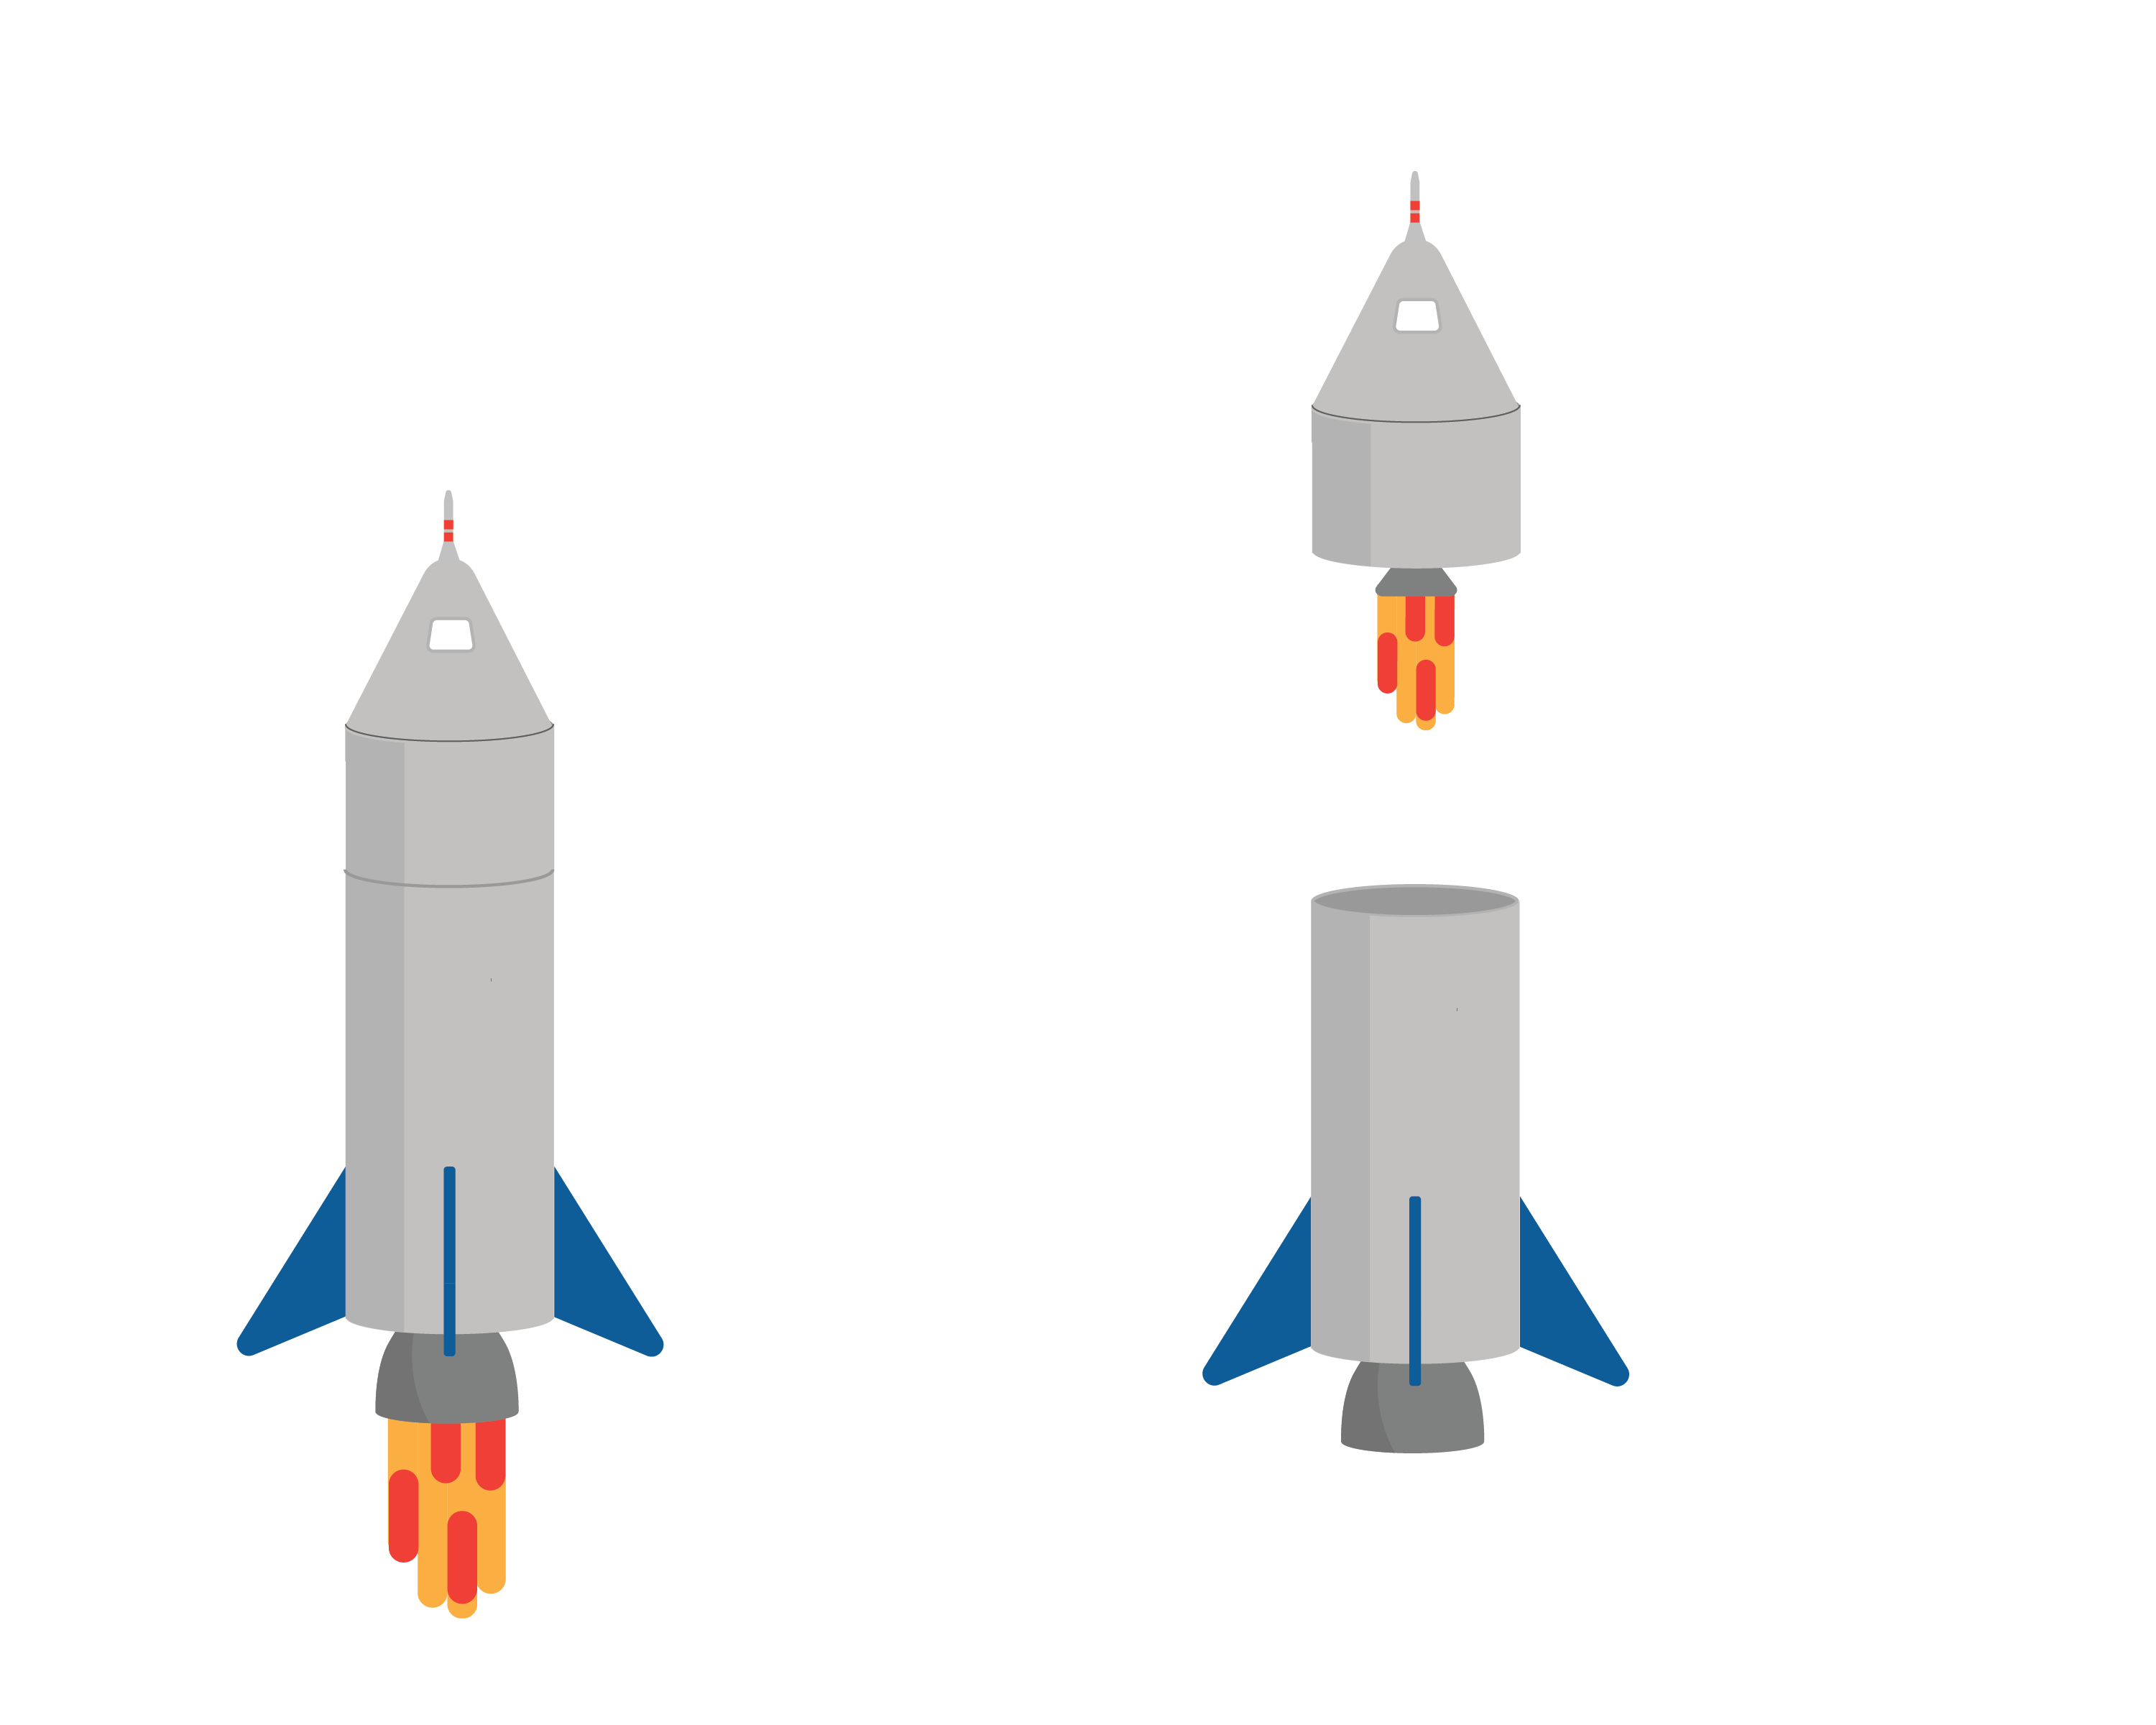
\includegraphics[width=0.75\textwidth]{stagingDual.png}


	However, the fuel needed increases X times to double the payload weight.

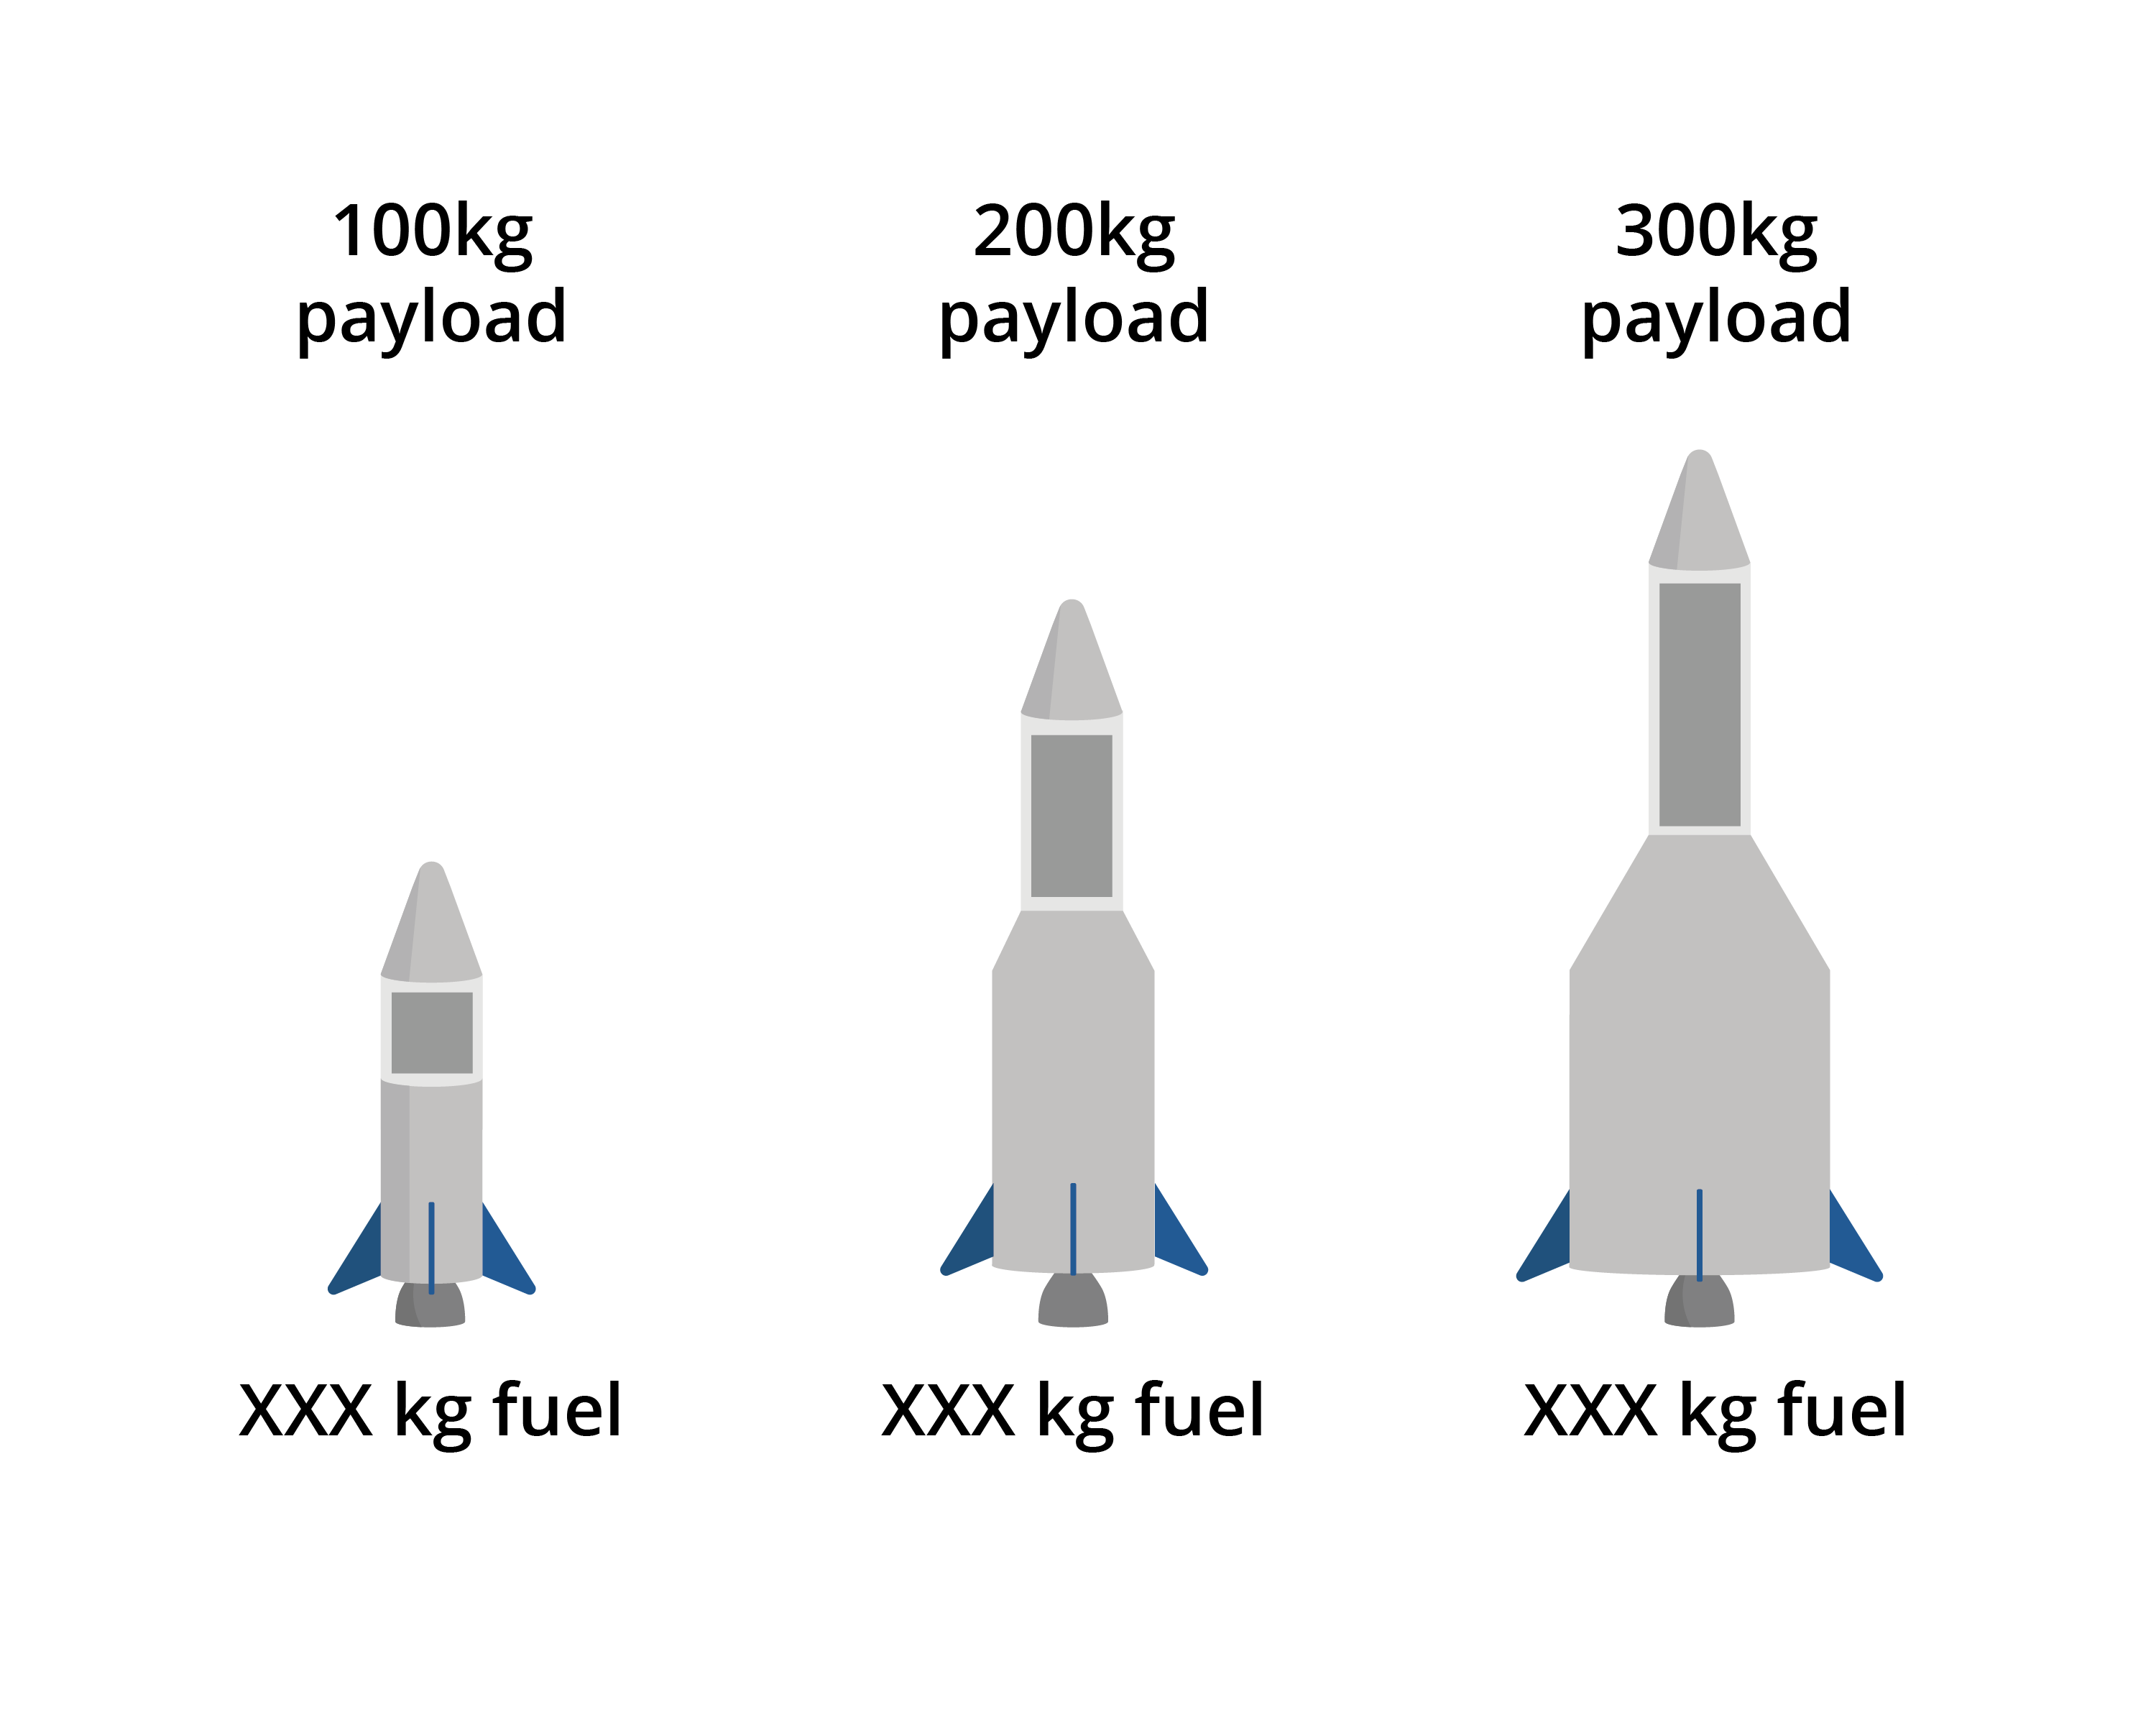
\includegraphics[width=0.75\textwidth]{rocketFuelWeight.png}


\section{Control in atmosphere}

There are several common ways that engineers have managed to control rockets' direction in the atmosphere. Usually, on-board sensors detect the orientation of the rocket, and can automatically adjust these controls to keep the rocket going the correct direction.

	
	One method is using \newterm{movable fins}. The fins work similar to control surfaces that we covered in the airplanes chapter. 



	Another method of control uses a \newterm{gimbaled engine}. [pros and cons]
	
	A more outdated method is using \newterm{vernier engines}, which are two smaller engines that control attitude. However, this adds a lot of weight to the rocket, so they are less frequently used today. [pros and cons]


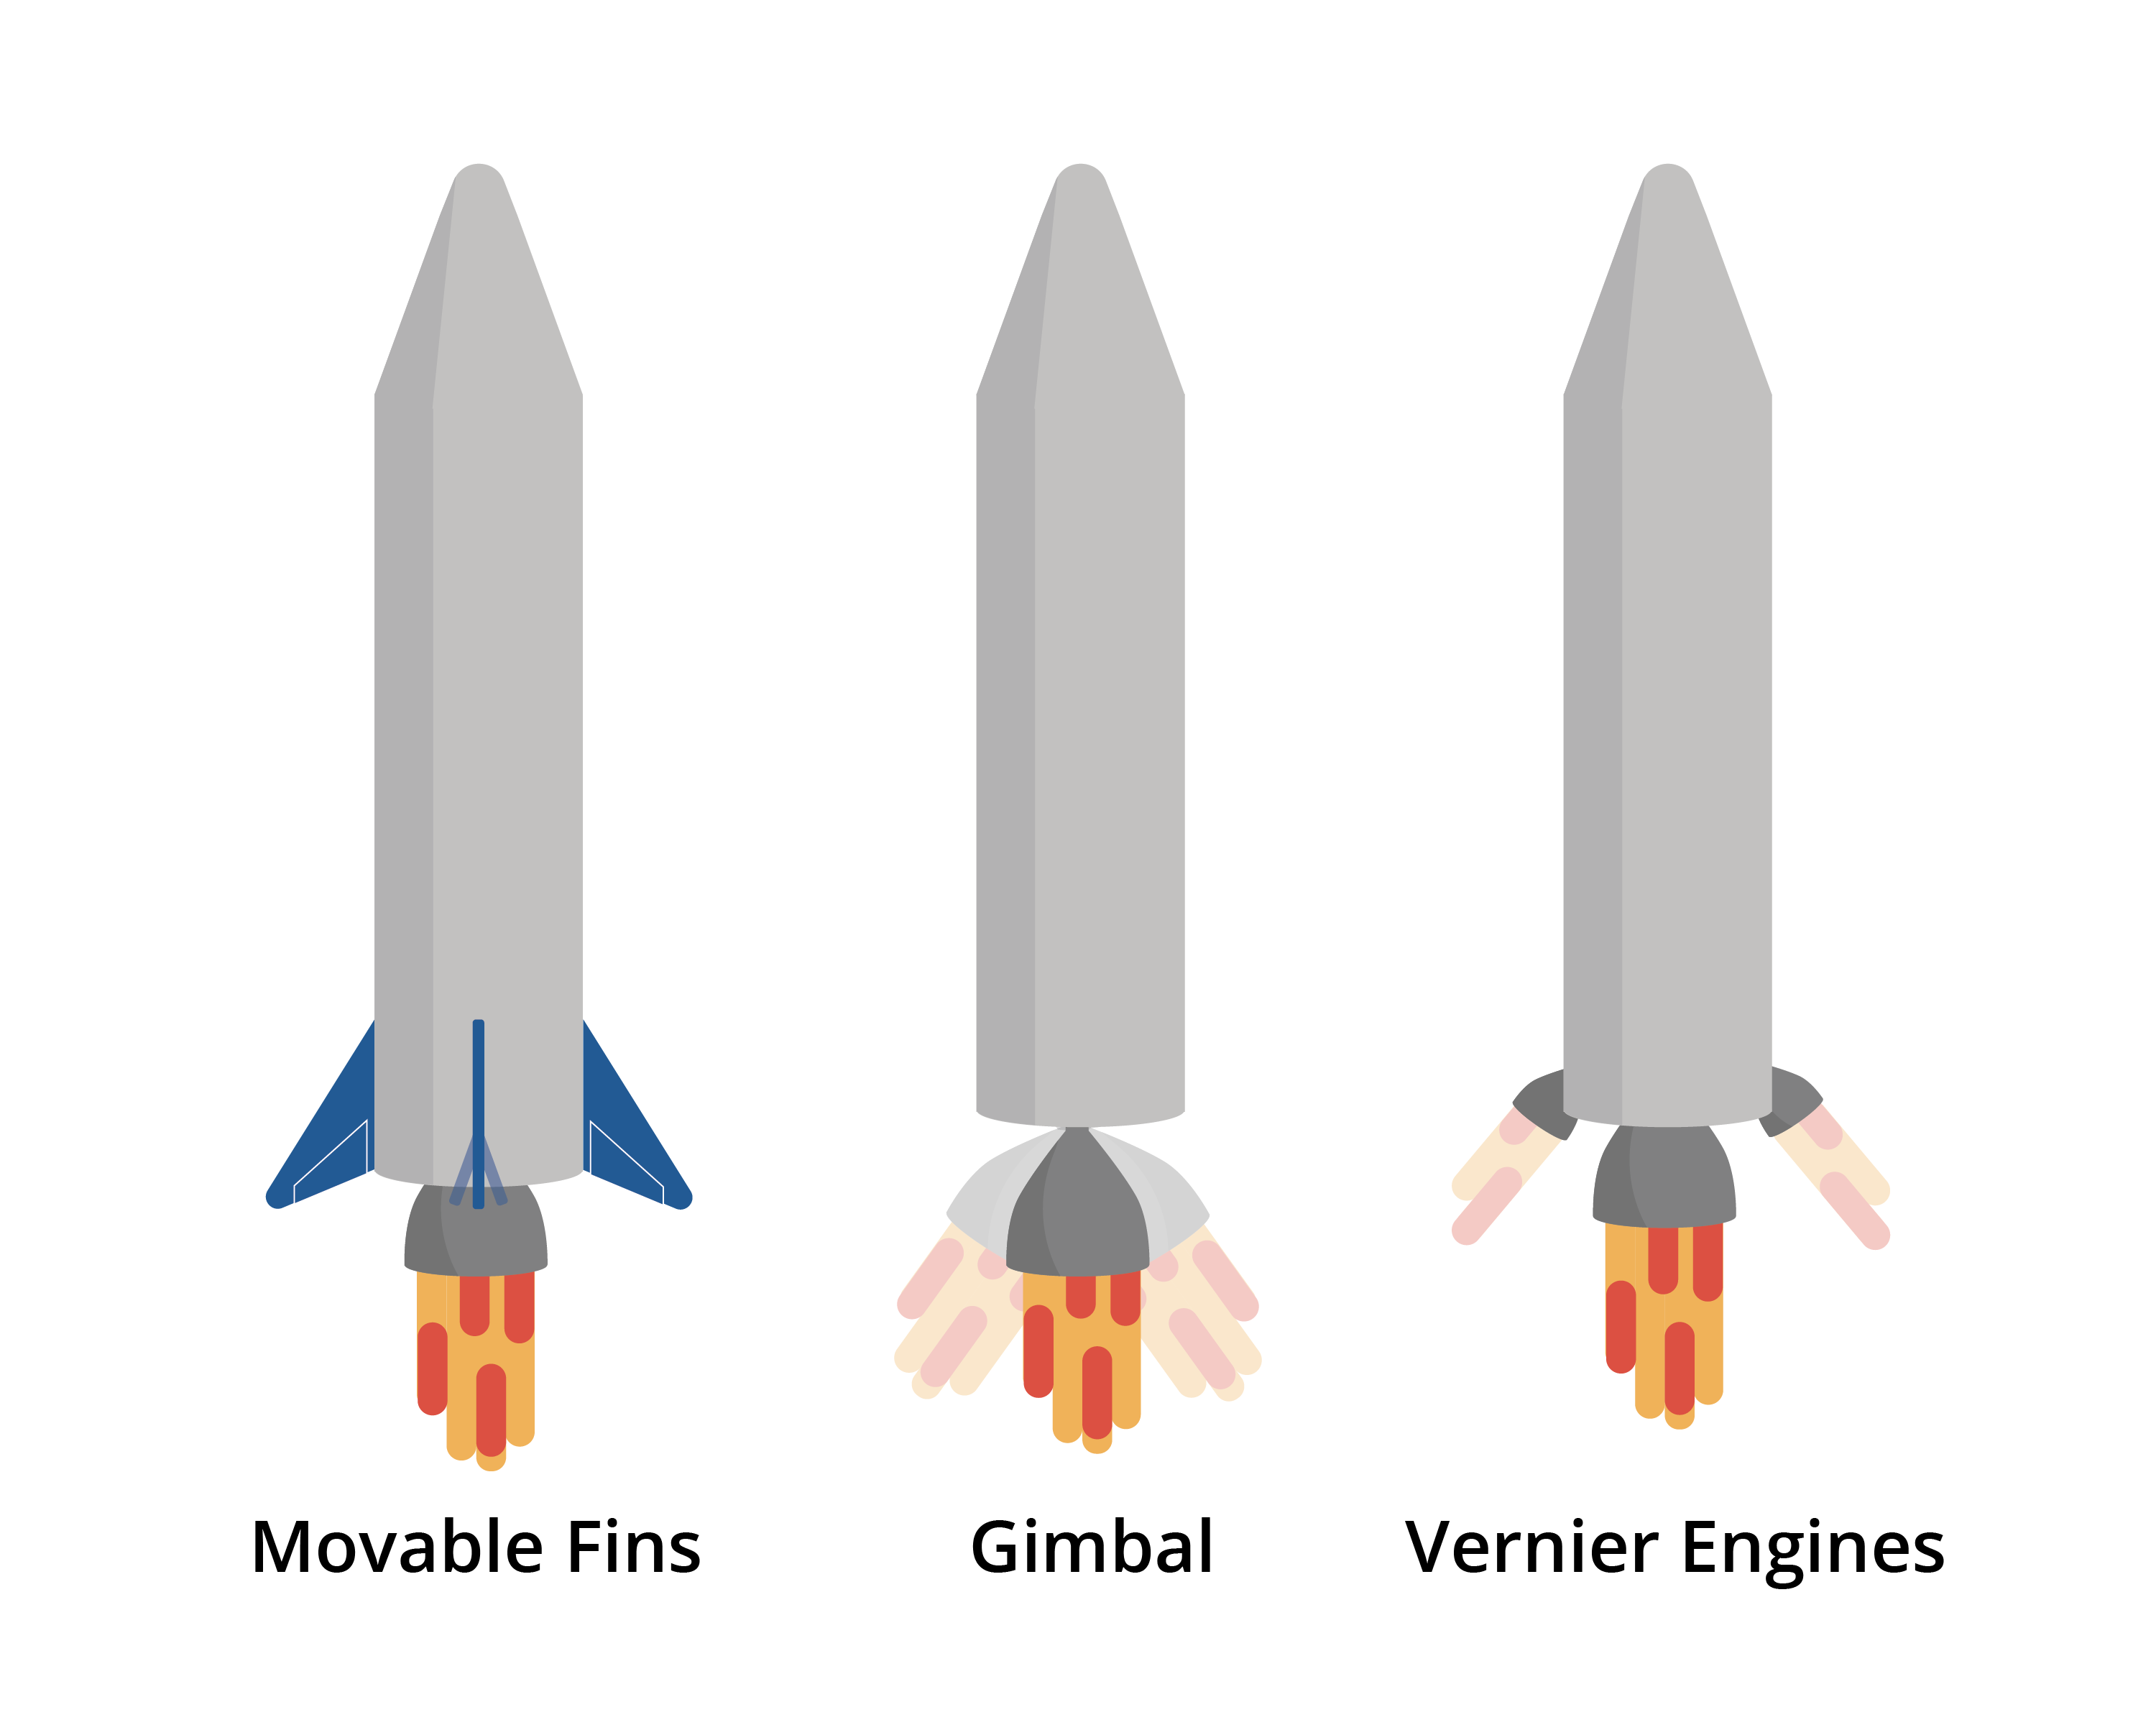
\includegraphics[width=0.75\textwidth]{control.png}


\section{Control in space}

The previous section describes ways that engineers control rockets in the atmosphere, but most rockets will end up in the vacuum of space. There are several common ways to adjust the orientation in space.

	One method is using \newterm{RCS thrusters}. An RCS, or reaction control system, is a series of small thrusters that are used to change the direction and position of a spacecraft. 

	Another method called \newterm{reaction wheels} uses angular momentum to rotate the spacecraft. By accelerating and decelerating wheels on three axes, the spacecraft can rotate in any direction.

	A third common attitude control technology is \newterm{magnetorquer}. Magnetorquers use electromagnets and the earth's magnetic field to adjust the orientation of the spacecraft. 


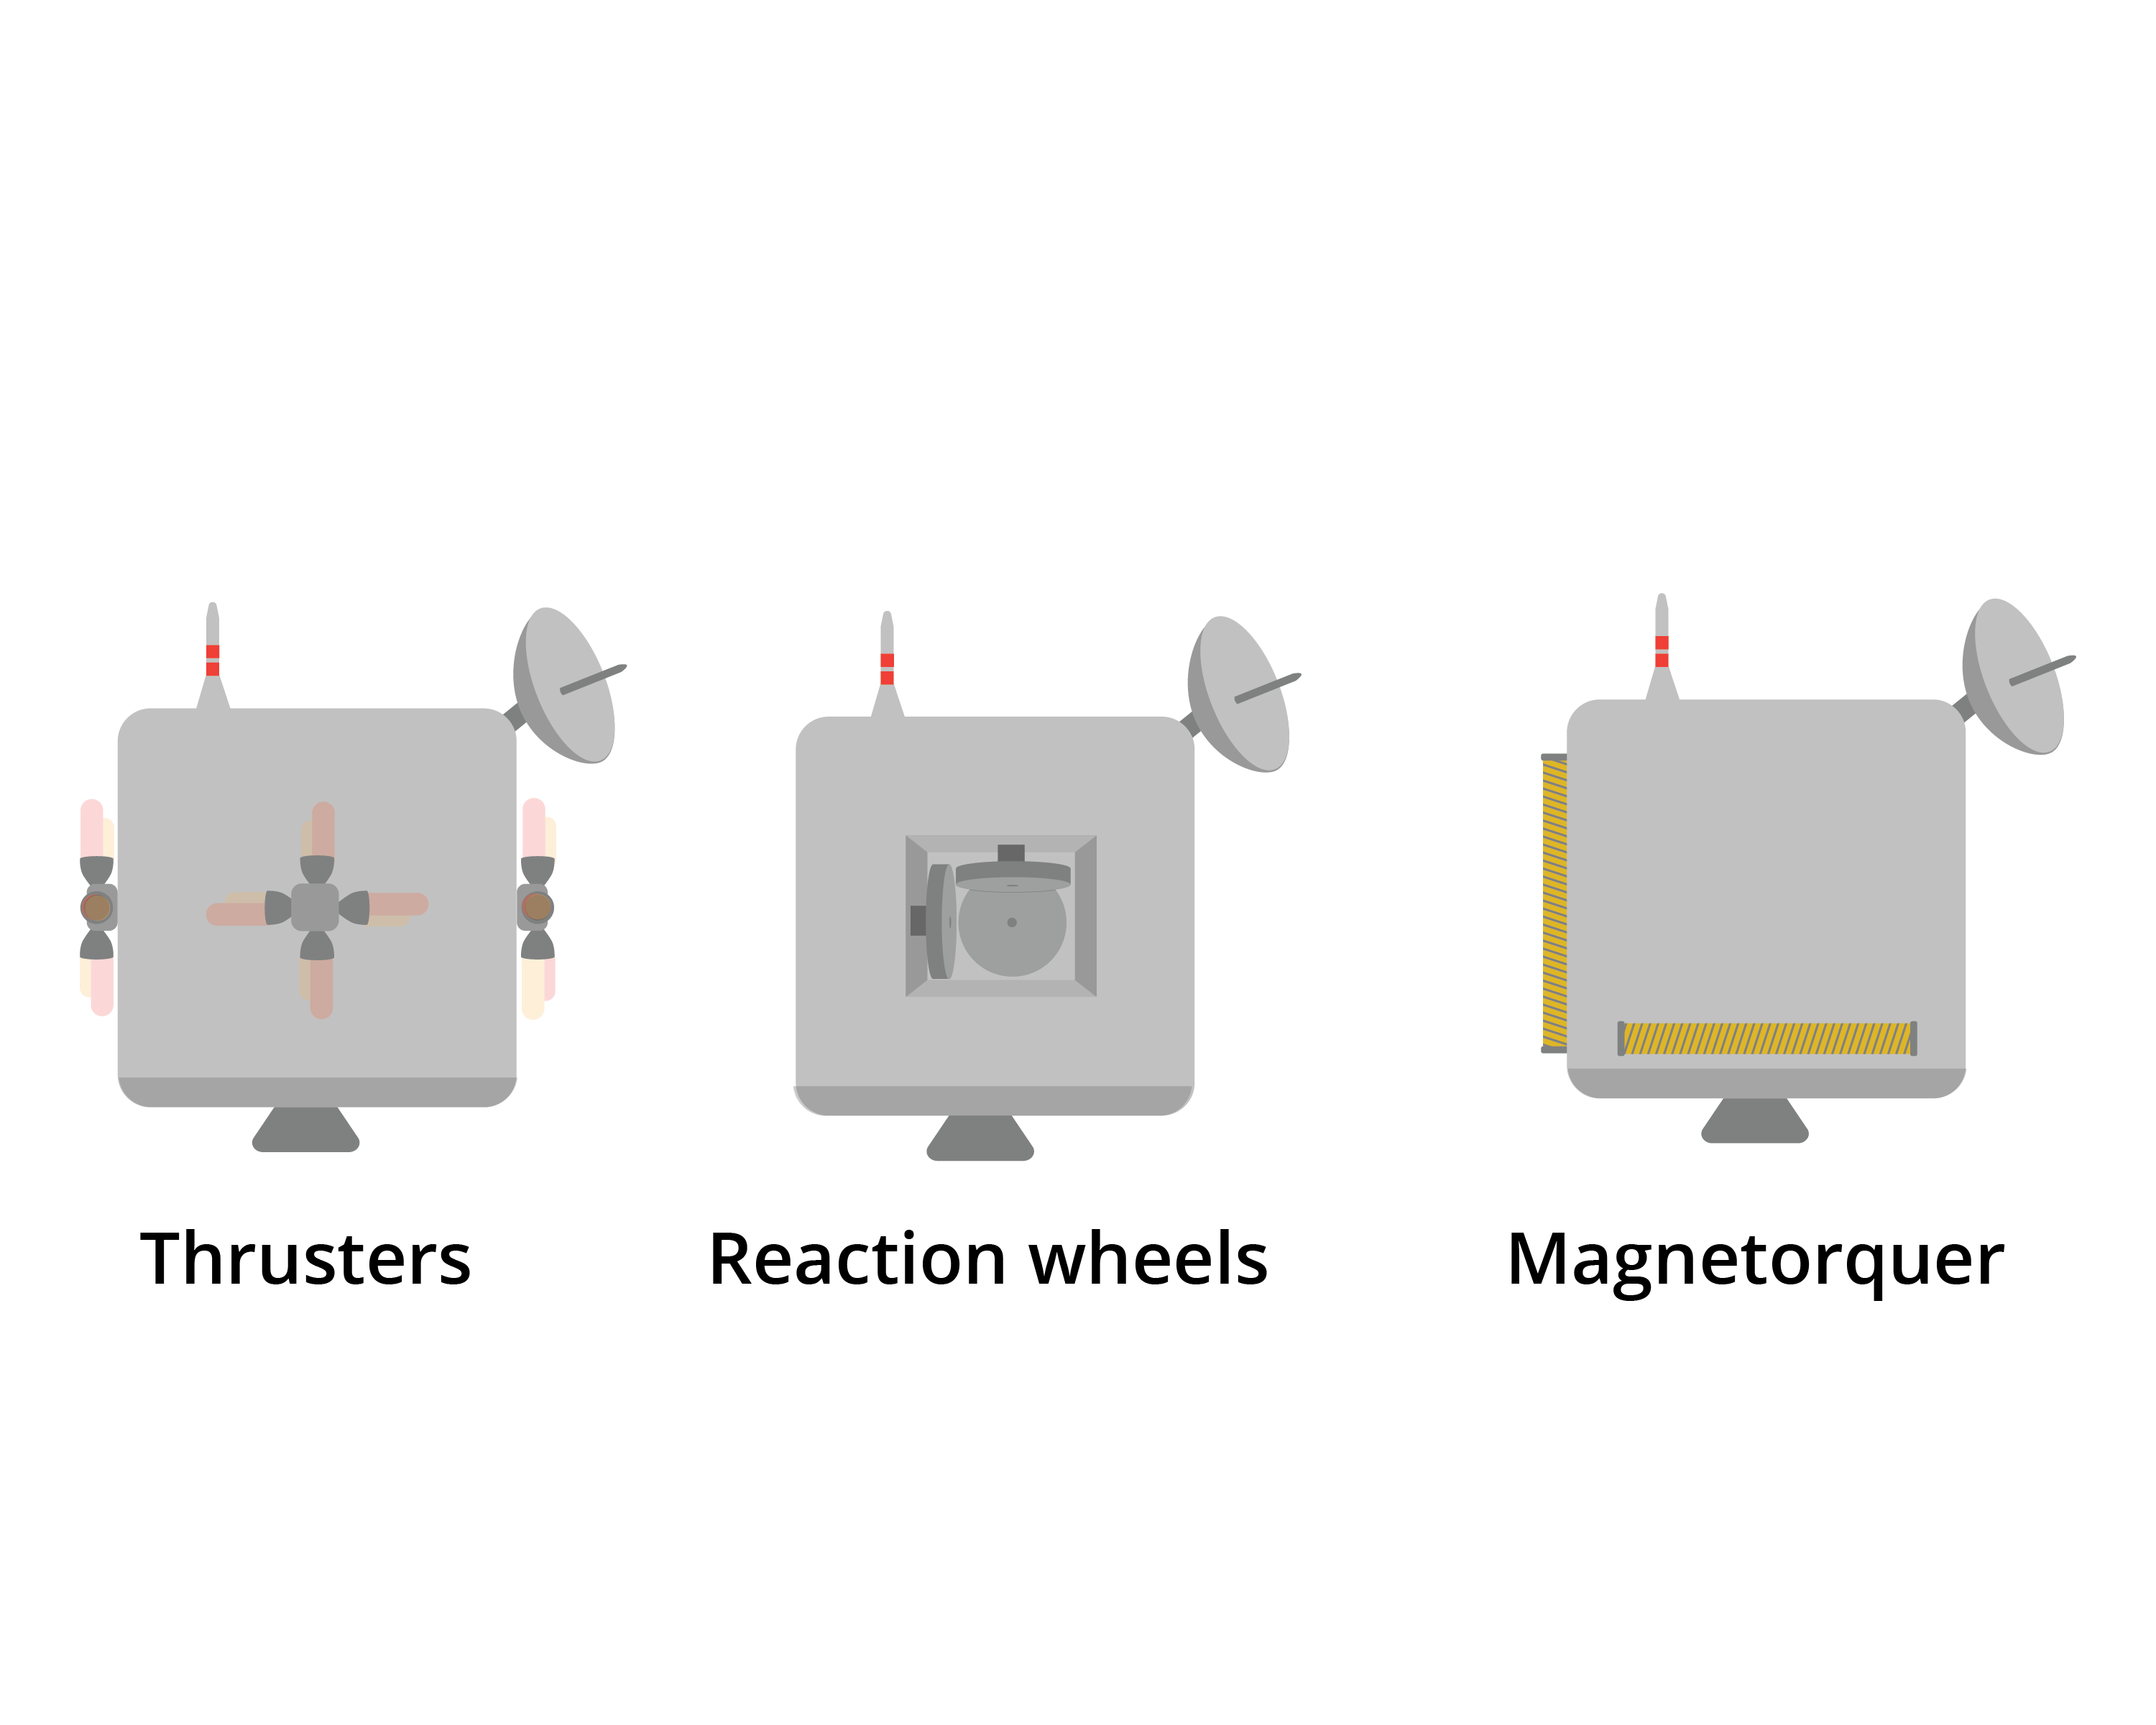
\includegraphics[width=0.75\textwidth]{controlSpace.png}



\section{Alternative propulsion}


One type of alternate propulsion is called a \newterm{solar sail}. Solar sails use lightweight reflective surfaces to use photons in space to propel the spacecraft without on-board fuel.


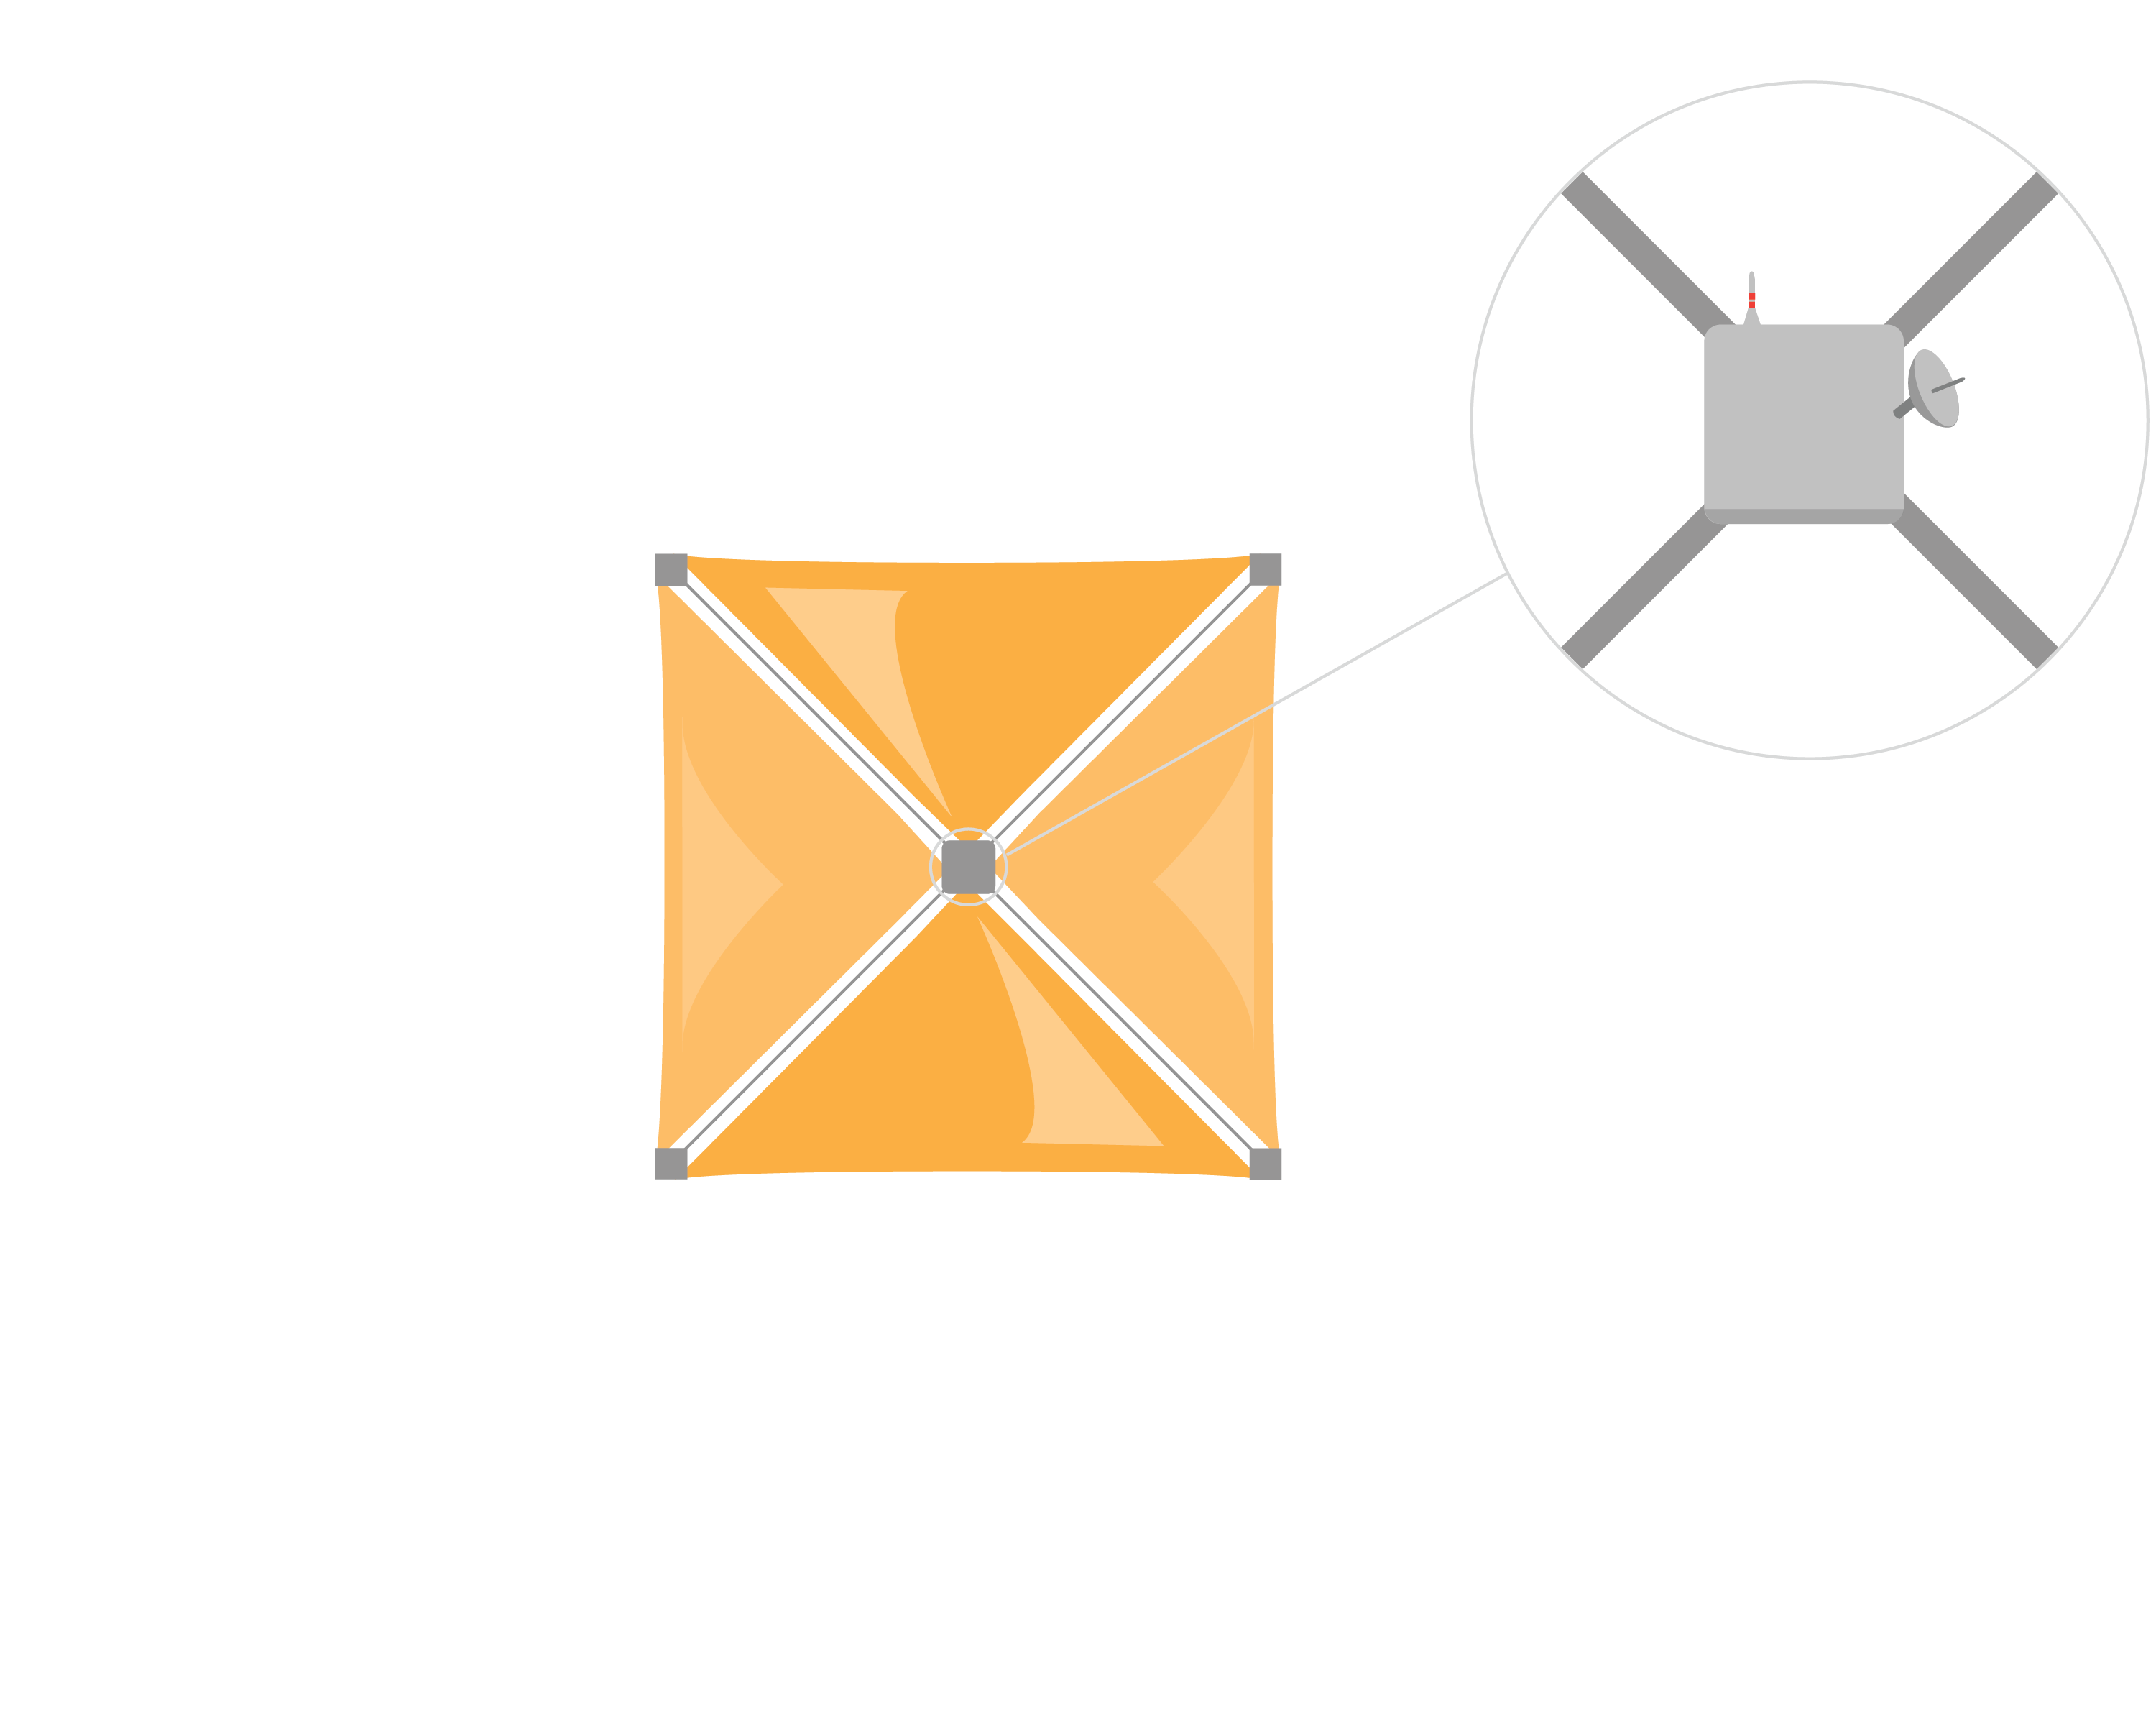
\includegraphics[width=0.75\textwidth]{solarSail.png}

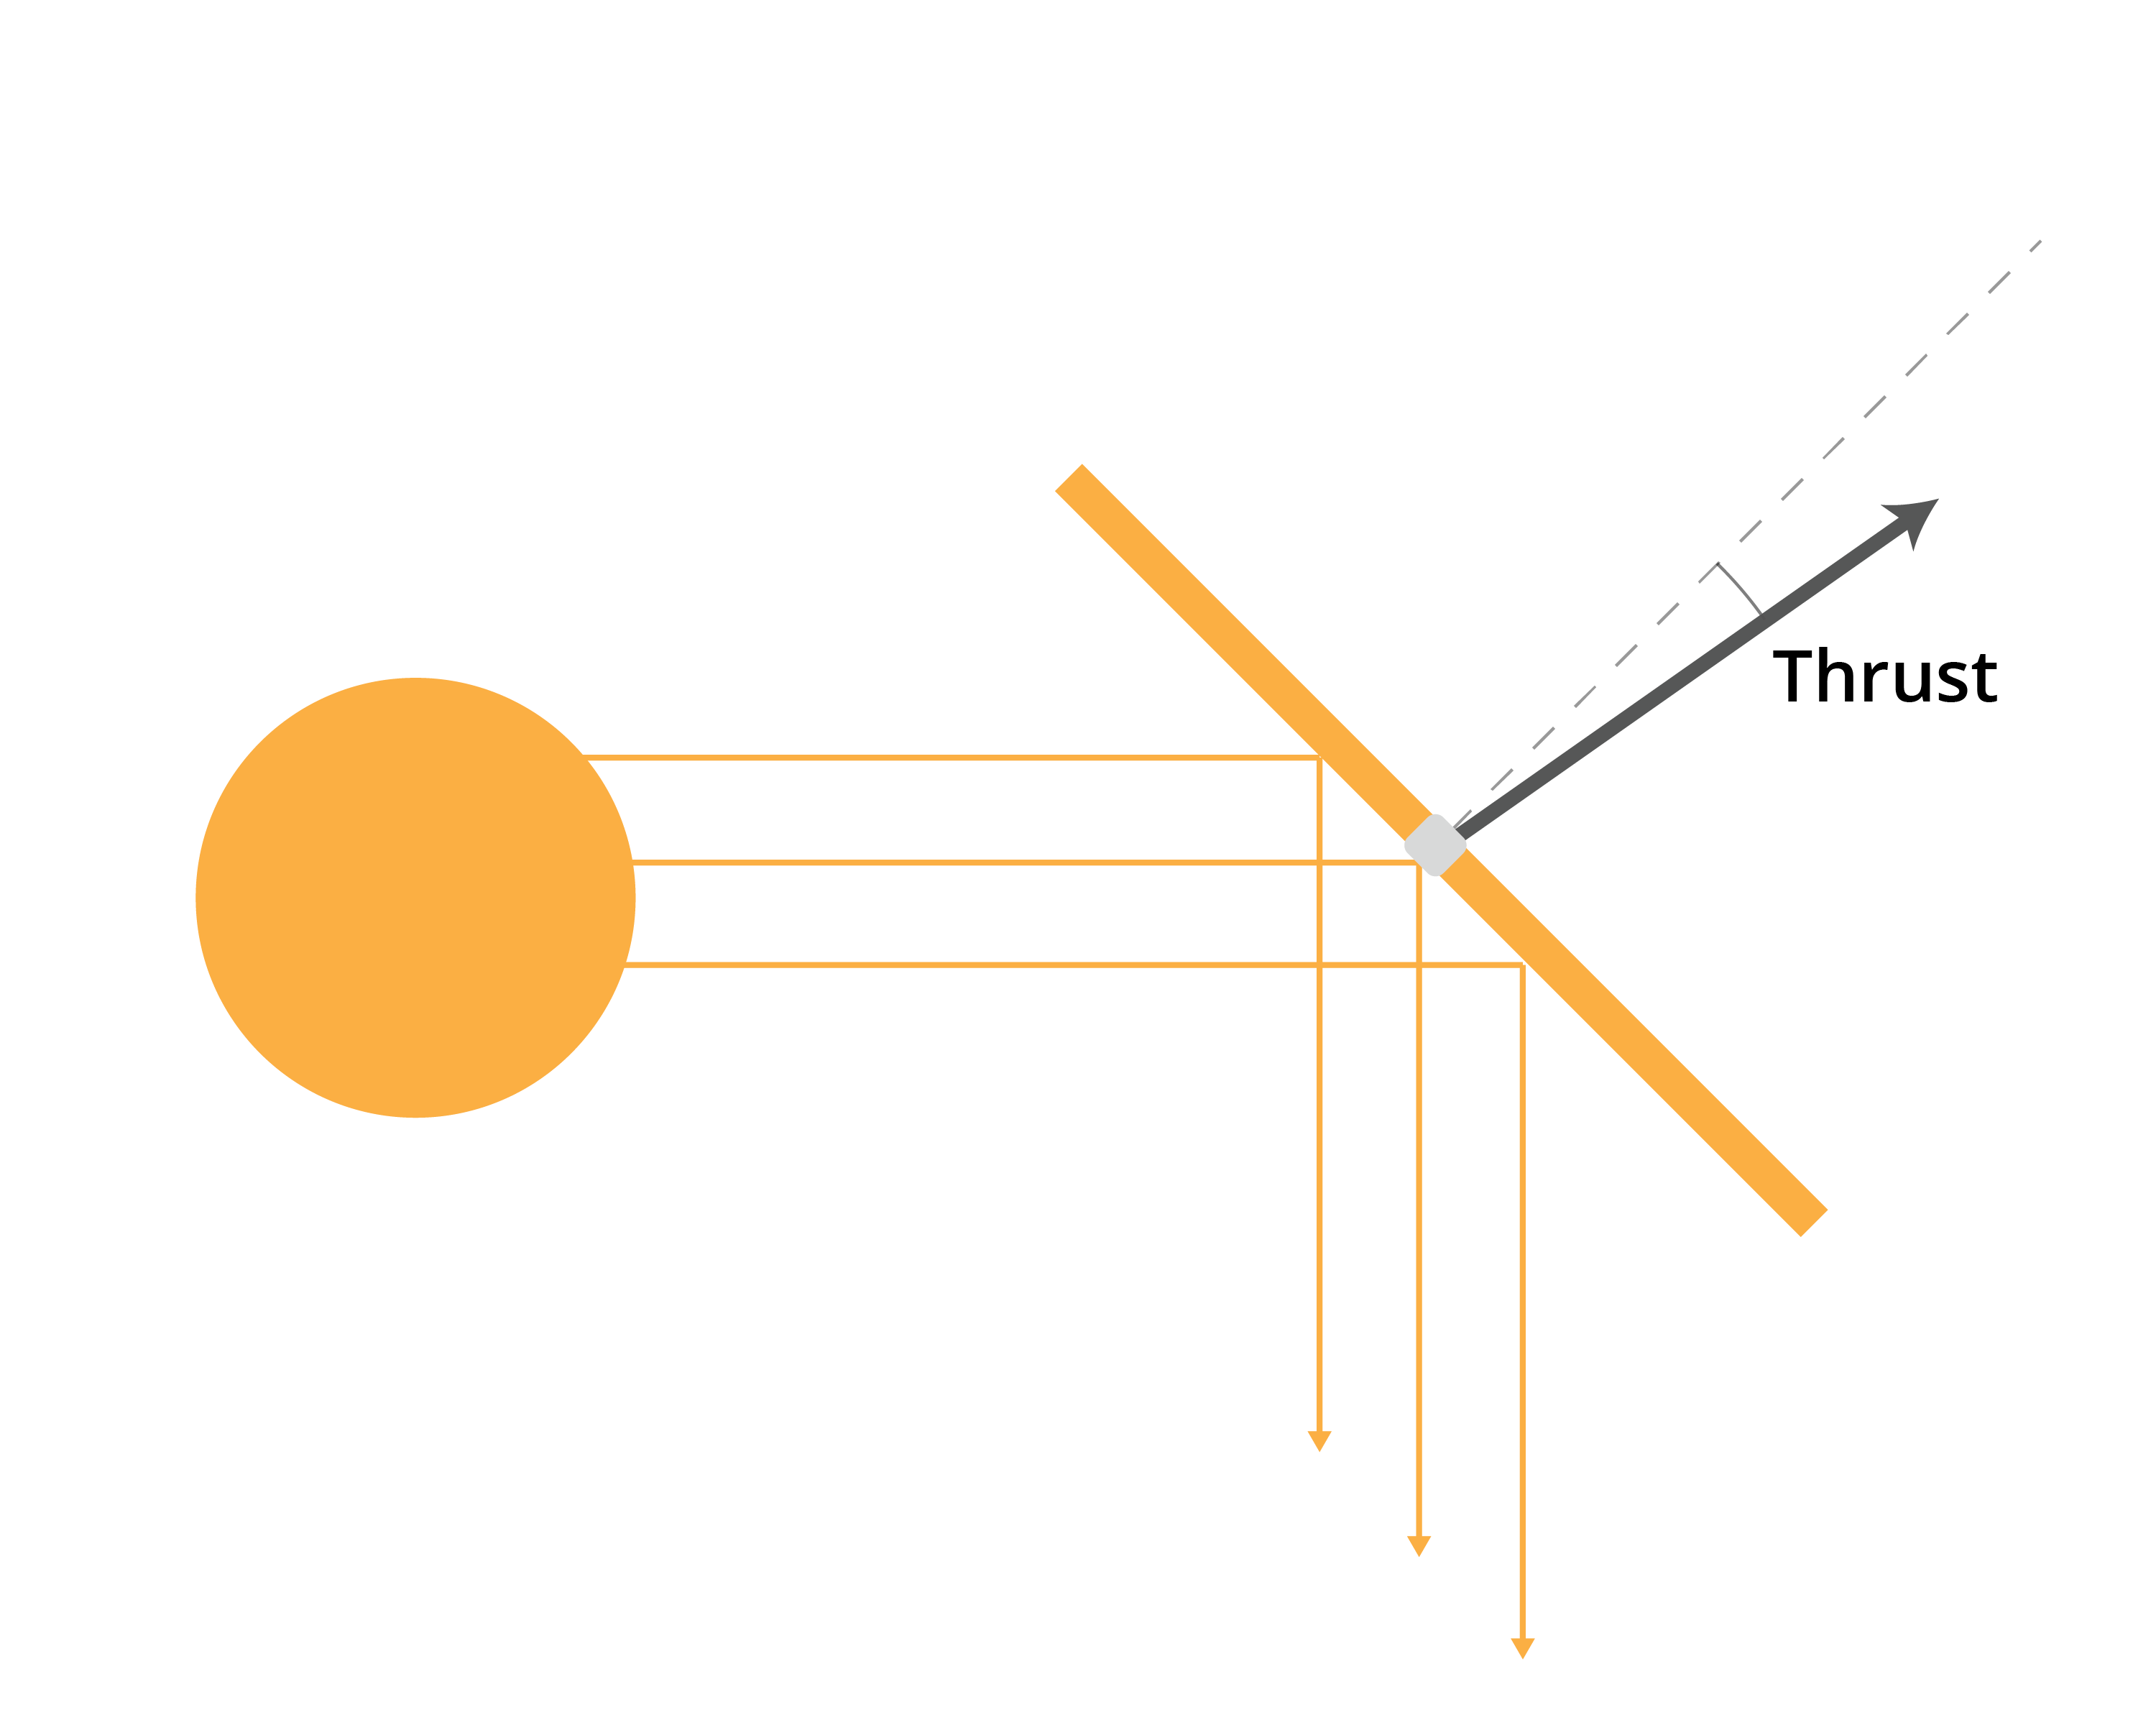
\includegraphics[width=0.75\textwidth]{solarSailDiagram.png}

Photons reflect off of the surface of the sail. However, since the surface is not perfectly reflective, some of those photons are absorbed, and they produce a horizontal equal and opposite reaction. That small force causes the net thrust to be slightly skewed away from a right angle to the sail.

\newterm{ion propulsion} 

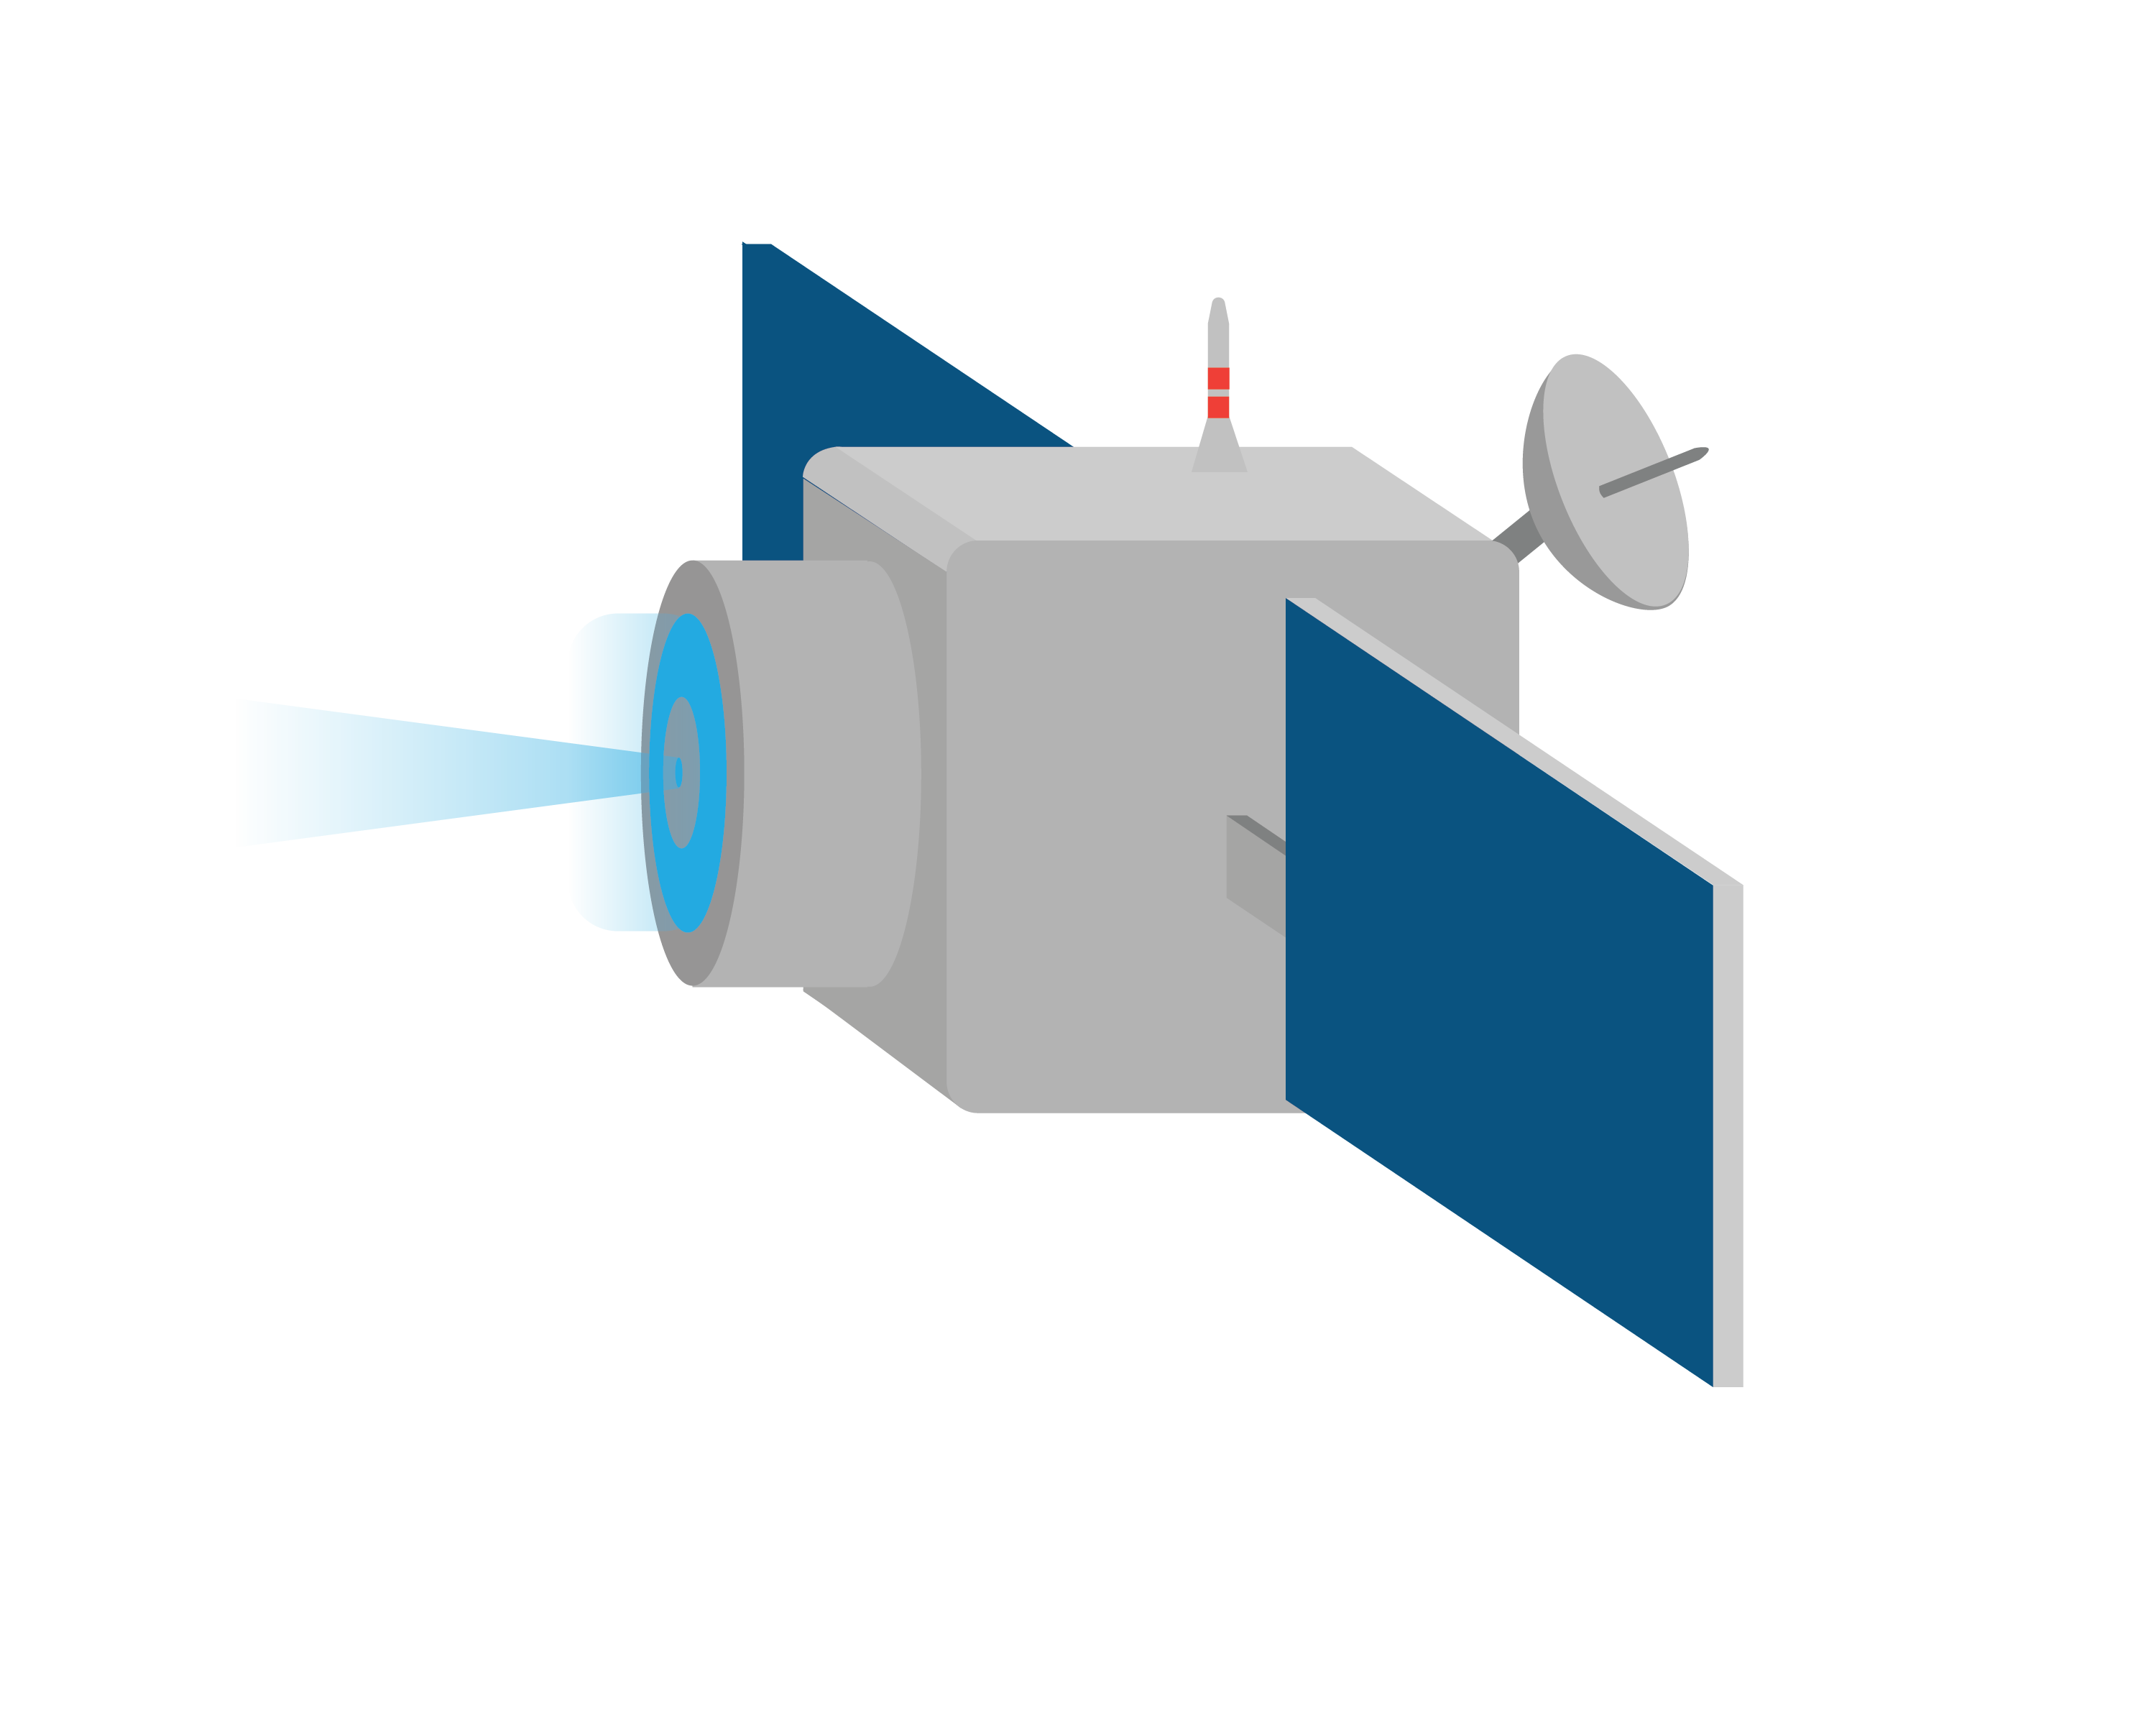
\includegraphics[width=0.75\textwidth]{ionThruster.png}





